\documentclass[letterpaper,12pt,oneside,final]{book}
%%
%%  Template de mémoire de maîtrise ou thèse de doctorat.
%%  Normalement, il n'est pas nécessaire de modifier ce document
%%  sauf pour changer les noms des fichiers à inclure.
%%
%%  Version: 2014-10-28
%%
%%  Accepte les caractères accentués dans le document (UTF-8).

\usepackage{balance}

\usepackage{enumitem}
\usepackage{hyperref}




\usepackage{graphicx}
%\usepackage{caption}
%\usepackage{subcaption}
\usepackage{color}
\usepackage{amsfonts}

\newenvironment{myindentpar}[1]%
{\begin{list}{}%
         {\setlength{\leftmargin}{#1}}%
         \item[]%
}
{\end{list}}

\newcommand{\hypobox}[1]{
        \begin{center}%
          \noindent
          \thicklines
          \setlength{\fboxsep}{8pt}%
          % \cornersize{0.2}
          \ovalbox{
            \begin{minipage}{3.0in}%
              % \textit{#1} 
              
            \end{minipage}
          } 
        \end{center}}

\newcommand{\bram}[1]{\textcolor{blue}{{\it [Bram: #1]}}}
\newcommand{\alex}[1]{\textcolor{red}{{\it [Alex: #1]}}}
\newcommand{\rqone}{How does expertise evolve in an open source project?}
\newcommand{\rqtwo}{How well does dimension 1 explain expertise?}
\newcommand{\rqthree}{How well does dimension 2 explain expertise?}




\usepackage[utf8]{inputenc}
%%
%% Support pour l'anglais et le français (français par défaut).
%\usepackage[cyr]{aeguill}
\usepackage{lmodern}      % Police de caractères plus complète et généralement indistinguable visuellement de la police standard de LaTeX (Computer Modern).
\usepackage[T1]{fontenc}  % Bon encodage des caractères pour qu'Acrobat Reader reconnaisse les accents et les ligatures telles que ffi.
\usepackage[frenchb,english]{babel} % le langage par défaut est le dernier de la liste, c'est-à-dire français
%%
%% Charge le module d'affichage graphique.
\usepackage{graphicx}
\usepackage{epstopdf}  % Permet d'utiliser des .eps avec pdfLaTeX.
%%
%% Recherche des images dans les répertoires.
\graphicspath{{./images/}{./dia/}{./gnuplot/}}
%%
%% Un float peut apparaître seulement après sa définition, jamais avant.
\usepackage{flafter,placeins}
%%
%% Utilisation de natbib pour les citations et la bibliographie.
\usepackage{natbib}
%%
%% Autres packages.
\usepackage{amsmath,color,soulutf8,longtable,colortbl,setspace,ifthen,xspace,url,pdflscape}
%%
%% Support des acronymes.
\usepackage[nolist]{acronym}
\onehalfspacing                % Interligne 1.5.
%%
%% Définition d'un style de page avec seulement le numéro de page à
%% droite. On s'assure aussi que le style de page par défaut soit
%% d'afficher le numéro de page en haut à droite.
\usepackage{fancyhdr}
\fancypagestyle{pagenumber}{\fancyhf{}\fancyhead[R]{\thepage}}
\renewcommand\headrulewidth{0pt}
\makeatletter
\let\ps@plain=\ps@pagenumber
\makeatother
%%
%% Module qui permet la création des bookmarks dans un fichier PDF.
%\usepackage[dvipdfm]{hyperref}
\usepackage{hyperref}
\usepackage{listings}
\usepackage{caption}  % Hyperlien vers la figure plutôt que son titre.
\makeatletter
\providecommand*{\toclevel@compteur}{0}
\makeatother
%%
%% Définitions spécifiques au format de rédaction de Poly.
\usepackage{MemoireThese}
%%
%% Définitions spécifiques à l'étudiant.
%% -----------------------------------
%% ---> A MODIFIER PAR L'ETUDIANT <---
%% -----------------------------------
%%
%% Commandes qui affichent le titre du document, le nom de l'auteur, etc.
\newcommand\monTitre{ON HISTORY-AWARE MULTI-ACTIVITY EXPERTISE MODELS}
\newcommand\monPrenom{Alexandre}
\newcommand\monNom{Courouble}
\newcommand\monDepartement{génie informatique et génie logiciel}
\newcommand\maDiscipline{génie informatique}
\newcommand\monDiplome{M}        % (M)aîtrise ou (D)octorat
\newcommand\anneeDepot{2017}
\newcommand\moisDepot{novembre}
\newcommand\monSexe{M}           % "M" ou "F"
\newcommand\PageGarde{N}         % "O" ou "N"
\newcommand\AnnexesPresentes{N}  % "O" ou "N". Indique si le document comprend des annexes.
\newcommand\mesMotsClef{Software Engineering, Mining Software Repositories, Software Expertise}
%%
%%  DEFINITION DU JURY
%%
%%  Pour la définition du jury, les macros suivantes sont definies:
%%  \PresidentJury, \DirecteurRecherche, \CoDirecteurRecherche, \MembreJury, \MembreExterneJury
%%
%%  Toutes les macros prennent 4 paramètres: Sexe (M/F), Prénom, Nom, Titres
\newcommand\monJury{\PresidentJury{M}{Giulio}{Antoniol}{Ph.~D.}\\
\DirecteurRecherche{M}{Bram}{Adams}{Ph.~D.}\\
\MembreJury{M}{Ettore}{Merlo}{Ph.~D.}}

\ifthenelse{\equal{\monDiplome}{M}}{
\newcommand\monSujet{Mémoire de maîtrise}
\newcommand\monDipl{Maîtrise ès sciences appliquées}
}{
\newcommand\monSujet{Thèse de doctorat}
\newcommand\monDipl{Philosophi\ae{} Doctor}
}
%%
%% Informations qui sont stockées dans un fichier PDF.
\hypersetup{
  pdftitle={\monTitre},
  pdfsubject={\monSujet},
  pdfauthor={\monPrenom{} \monNom},
  pdfkeywords={\mesMotsClef},
  bookmarksnumbered,
  pdfstartview={FitV},
  hidelinks,
  linktoc=all
}
%%
%% Il y a un document par chapitre du mémoire.
%%
\begin{document}
%%
%% Page de titre du mémoire.
\frontmatter
% Compte optionellement la page de garde dans la pagination.
\ifthenelse{\equal{\PageGarde}{O}}{\addtocounter{page}{1}}{}
\thispagestyle{empty}%
\begin{center}%
\vspace*{\stretch{1}}
UNIVERSITÉ DE MONTRÉAL\\
\vspace*{\stretch{1}}
\MakeUppercase{\monTitre}\\
\vspace*{\stretch{1}}
\MakeUppercase{\monPrenom~\monNom}\\
DÉPARTEMENT DE \MakeUppercase{\monDepartement}\\
ÉCOLE POLYTECHNIQUE DE MONTRÉAL\\
\vspace*{\stretch{1}}
\ifthenelse{\equal{\monDiplome}{M}}{MÉMOIRE PRÉSENTÉ}{THÈSE PRÉSENTÉE} EN VUE DE L'OBTENTION\\
DU DIPLÔME DE \MakeUppercase{\monDipl}\\
(\MakeUppercase{\maDiscipline})\\
\MakeUppercase{\moisDepot} \anneeDepot
\end{center}%
\vspace*{\stretch{1}}
\copyright~\monPrenom~\monNom, \anneeDepot.
%%
%% Identification des membres du jury.
%%
\newpage\thispagestyle{empty}%
\begin{center}%
\vspace*{\stretch{2}}
\ul{UNIVERSITÉ DE MONTRÉAL}\\
\vspace*{\stretch{1}}
\ul{ÉCOLE POLYTECHNIQUE DE MONTRÉAL}\\
\vspace*{\stretch{2}}
Ce\ifthenelse{\equal{\monDiplome}{M}}{~mémoire intitulé}{tte thèse intitulée}:\\
\vspace*{\stretch{1}}
\MakeUppercase{\monTitre}\\
\vspace*{\stretch{2}}
\end{center}%
\begin{flushleft}
présenté\ifthenelse{\equal{\monDiplome}{M}}{}{e}
par:~\ul{\mbox{\MakeUppercase{\monNom} \monPrenom}}\\
en vue de l'obtention du diplôme de:~\ul{\mbox{\monDipl}}\\
a été dûment accepté\ifthenelse{\equal{\monDiplome}{M}}{}{e} par le jury d'examen constitué de:\end{flushleft}
\vspace*{\stretch{2}}
\monJury
%%
\pagestyle{pagenumber}%
%% Dédicace
%%
%% La dédicace est un hommage que l'auteur souhaite
%% rendre à une ou plusieurs personnes de son choix.
%%
\chapter*{DEDICATION}\thispagestyle{headings}
\addcontentsline{toc}{compteur}{DEDICATION}
\begin{flushright}
  \itshape
  To all friends at the lab,\\
  I will miss you\ldots
\end{flushright}
          % Dédicace du document.
% Remerciements
%
%   Grâce aux remerciements, l'auteur attire l'attention du lecteur
% sur l'aide que certaines personnes lui ont apportée, sur leurs
% conseils ou sur toute autre forme de contribution lors de la
% réalisation de son mémoire. Le cas échéant, c'est dans cette section
% que le candidat doit témoigner sa reconnaissance à son directeur de
% recherche, aux organismes dispensateurs de subventions ou aux
% entreprises qui lui ont accordé des bourses ou des fonds de
% recherche.
\chapter*{ACKNOWLEDGEMENTS }\thispagestyle{headings}
\addcontentsline{toc}{compteur}{ACKNOWLEDGEMENTS }
%
In the acknowledgements, the author points out the help that various people have provided, including advice or any other type of contribution as the author carried out their research. As appropriate, this is the section where the candidate must thank their thesis or dissertation supervisor, grant-awarding organizations, or companies that provided bursaries or research funds. 

If the thesis or dissertation is in French and students wish to thank someone in particular in English, they must insert a second page and title it in English (i.e., “Acknowledgments”).  If the thesis or dissertation is in English and students wish to thank someone in particular in French, they must insert a second page and title it in French (i.e., “Remerciements”).

     % Remerciements.
% Résumé du mémoire.
%
%   Le résumé est un bref exposé du sujet traité, des objectifs visés,
% des hypothèses émises, des méthodes expérimentales utilisées et de
% l'analyse des résultats obtenus. On y présente également les
% principales conclusions de la recherche ainsi que ses applications
% éventuelles. En général, un résumé ne dépasse pas quatre pages.
%
%   Le résumé doit donner une idée exacte du contenu du mémoire ou de la thèse. Ce ne
% peut pas être une simple énumération des parties du document, car il
% doit faire ressortir l'originalité de la recherche, son aspect
% créatif et sa contribution au développement de la technologie ou à
% l'avancement des connaissances en génie et en sciences appliquées.
% Un résumé ne doit jamais comporter de références ou de figures.

\chapter*{RÉSUMÉ}\thispagestyle{headings}
\addcontentsline{toc}{compteur}{RÉSUMÉ}

Durant l'évolution d'un projet de logiciel, les contributions individuelles d'un developeur present dans le projet vont lentement se faire remplacer par les contributions d'autre dévelopeurs. Ceci engendrera l'érosion de l'empreinte des contributions de ce developeur. Bien que les connaissances de ce dévelopeur n'ont pas disparu du jour au lendemain, pour une personne externe au projet, l'expertise de ce developeur est devenue invisible. 

Grace à une étude empirique sur une periode de 5 années de developement de Linux, nous étudions le phénomène de l'érosion de l'expertise en créant un modèle bidimentionnel. La première dimention de notre modèle prend en compte les différentes activités entreprises par les membres de la communauté de développement de Linux, comme les contributions en termes de code, les contributions aux revues de code soumit par d'autre dévelopeurs, ou encore la soumission de code d'autres dévelopeurs en amont. La deuxiéme dimention de notre modèle prend en compte l'historique des contributions citées plus haut pour chaque dévelopeurs. 

En applicant ce modèle, nous decouvrons que, bien que les empreintes de contributions de certain dévelopeurs diminuent avec le temps, leurs expertise survit grace à leurs implications dans les divereses activités mentionées plus haut. 

% Dans ce mémoire, nous expliquons les differentes étapes entreprises pour la création de ce modèle. Premiérement, nous fournissons

% \alex{more}      % Résumé du sujet en français.
% Abstract
%
%   Résumé de la recherche écrit en anglais sans être
% une traduction mot à mot du résumé écrit en français.

\chapter*{ABSTRACT}\thispagestyle{headings}
\addcontentsline{toc}{compteur}{ABSTRACT}
%
\begin{otherlanguage}{english}

% Written in English, the abstract is a brief summary similar to the previous
% section {\selectlanguage{frenchb}(Résumé)}.  However, this section is not a
% word for word translation of the French.


As software evolves, a developer's contributions will gradually vanish as they are being replaced by other developers' code, slowly eroding the developer's footprint in the software project. Even though this developer's knowledge of the file did not disappear overnight, to outsiders, the developer and her expertise have become invisible. Through an empirical study on 5 years of Linux development history, this paper analyses this phenomenon of expertise erosion by building a 2-dimensional model of developer expertise involving a range of developer activities and involving activity data on more than one release. Using these models, we found that although many Linux maintainers' own coding footprint has regressed over time, their expertise is perpetuated through involvement in other development activities such as patch reviews and committing upstream on behalf of other developers. Considering such activities over time further improves the expertise models.

\end{otherlanguage}
          % Résumé du sujet en anglais.

{\setlength{\parskip}{0pt}
%%
%% Table des matières.
\renewcommand\contentsname{TABLE OF CONTENTS}
\tableofcontents
%%
%% Liste des tableaux.
\renewcommand\listtablename{LIST OF TABLES}
\listoftables
%%
%% Table des figures.
\renewcommand\listfigurename{LIST OF FIGURES}
\listoffigures
%%
%% Liste des annexes au besoin.
}

% Liste des sigles et abbréviations
\newcommand\abbrevname{LIST OF SYMBOLS AND ABBREVIATIONS}
\chapter*{\abbrevname}
\addcontentsline{toc}{compteur}{\abbrevname}
\pagestyle{pagenumber}
%
\begin{acronym}
  \acro{LOC}{Lines of Code}
  \acro{SCM}{Source Code Managment}
  \acro{OSS}{Open Source Software}
  \acro{MSR}{Mining Software Repositories}
\end{acronym}
%
\begin{longtable}{lp{5in}}
LOC		   & Lines of Code\\
SCM		   & Source Code Managment\\
OSS		   & Open Source Software\\
MSR 	   & Mining Software Repositories\\
\end{longtable}

       % Liste des sigles et abréviations.
\ifthenelse{\equal{\AnnexesPresentes}{O}}{\listofappendices}{}
\mainmatter
%   Dans l'introduction, on présente le problème étudié et les buts
% poursuivis. L'introduction permet de faire connaître le cadre de la
% recherche et d'en préciser le domaine d'application. Elle fournit
% les précisions nécessaires en ce qui concerne le contexte de
% réalisation de la recherche, l'approche envisagée, l'évolution de
% la réalisation. En fait, l'introduction présente au lecteur ce
% qu'il doit savoir pour comprendre la recherche et en connaître la
% portée.
\Chapter{INTRODUCTION}\label{sec:Introduction}  






As an answer to the risks associated with employee turn over in software engineering organizations, researchers have attempted to establish models capable of finding experts in certain code areas. By recommending experienced developers, these models would ease the difficulty of replacing current experts as they leave the organization. 


Introduced in the early 2000s, these models were using two simple metrics to assess expertise: number of \ac{LOC} and number of commits. 


However, using these metrics to measure expertise on \textit{modern} large scale software project does not yield accurate results. we believe that, as the teams behind large software projects increase in size, these models tend to lose accuracy. 

The Linux Kernel, for instance, is a 26-year-old project that has experienced a drastic growth in terms of code base and in terms of developer community. Wanting to keep a high standard of code quality and a fast release system, the community had to implement a hierarchical contribution system. In this contribution system, some developers are responsible for the maintenance of their subsystems. These developers, or maintainers, are trusted by the rest of the Linux community to be skilled enough to ensure the durability of their subsystem. This trust was acquired by contributing to the subsystem over the years. However, when trying to use traditional expertise determining metrics in the linux kernel, maintainers are rarely recomended. 


We believe that previous expertise models fail to take into account some critical aspect of large scale software development. As subsystems become larger and welcome more contributors, maintainers have to dedicate more of their time reviewing other developers' contributions to maintain code quality. This shift towards a managerial position is usually followed by a drop in code contributions by that person. This implies that, in the eye of a model looking at only \ac{LOC} and commits, the maintainer will lose expertise. 


We introduce a new expertise model adapted to large software organization like the Linux community. Our model is better suited for the Linux community because it takes into account all the activities undertaken by both maintainers and developers. This thesis provides an in-depth description of the different steps necessary for the creation of this model.





\section{Definitions and Concepts}  % environ 2-3 pages


\subsection{The Anatomy of a Git Commit}
\label{sec:commit_anatomy}

A git commit is a fundamental concept in the scope of this research and for the understanding of git in general. The changes brought to source code by developers are contained in a \textit{commit}. If a developer is tasked to fix a bug or to create a new feature in a project, she will have to modify the source code in order to implement these changes. When a developer feels ready to share these changes, she can apply them to the repository in the form of a git commit. The changes are reprented in the \textit{commit diff}, which contains the exact lines to be removed (-) or added (+) in the source code. Git uses the +/- lines to modify the repository of someone who \textit{pulled} the changes form the developer as depicted in \autoref{fig:commit_anatomy}. 

Furthermore, commits contain an array of metadata regarding the changes committed, all of which is accessible to anyone with a copy of the repository through a handful of builtin commands. For example, git log returns information about the past commits in the repository. \autoref{fig:commit_anatomy} shows one commit in the output printed by the following command: \texttt{git log -{}-pretty=fuller -{}-patch}, where the \texttt{-{}-pretty=fuller} shows more information and \textit{-{}-patch} shows the commit diff. There are three main parts to the commit as seen in the image: the header, the  message, and the diff.

The header contains the following data points:

\begin{figure}[htb]
\centering
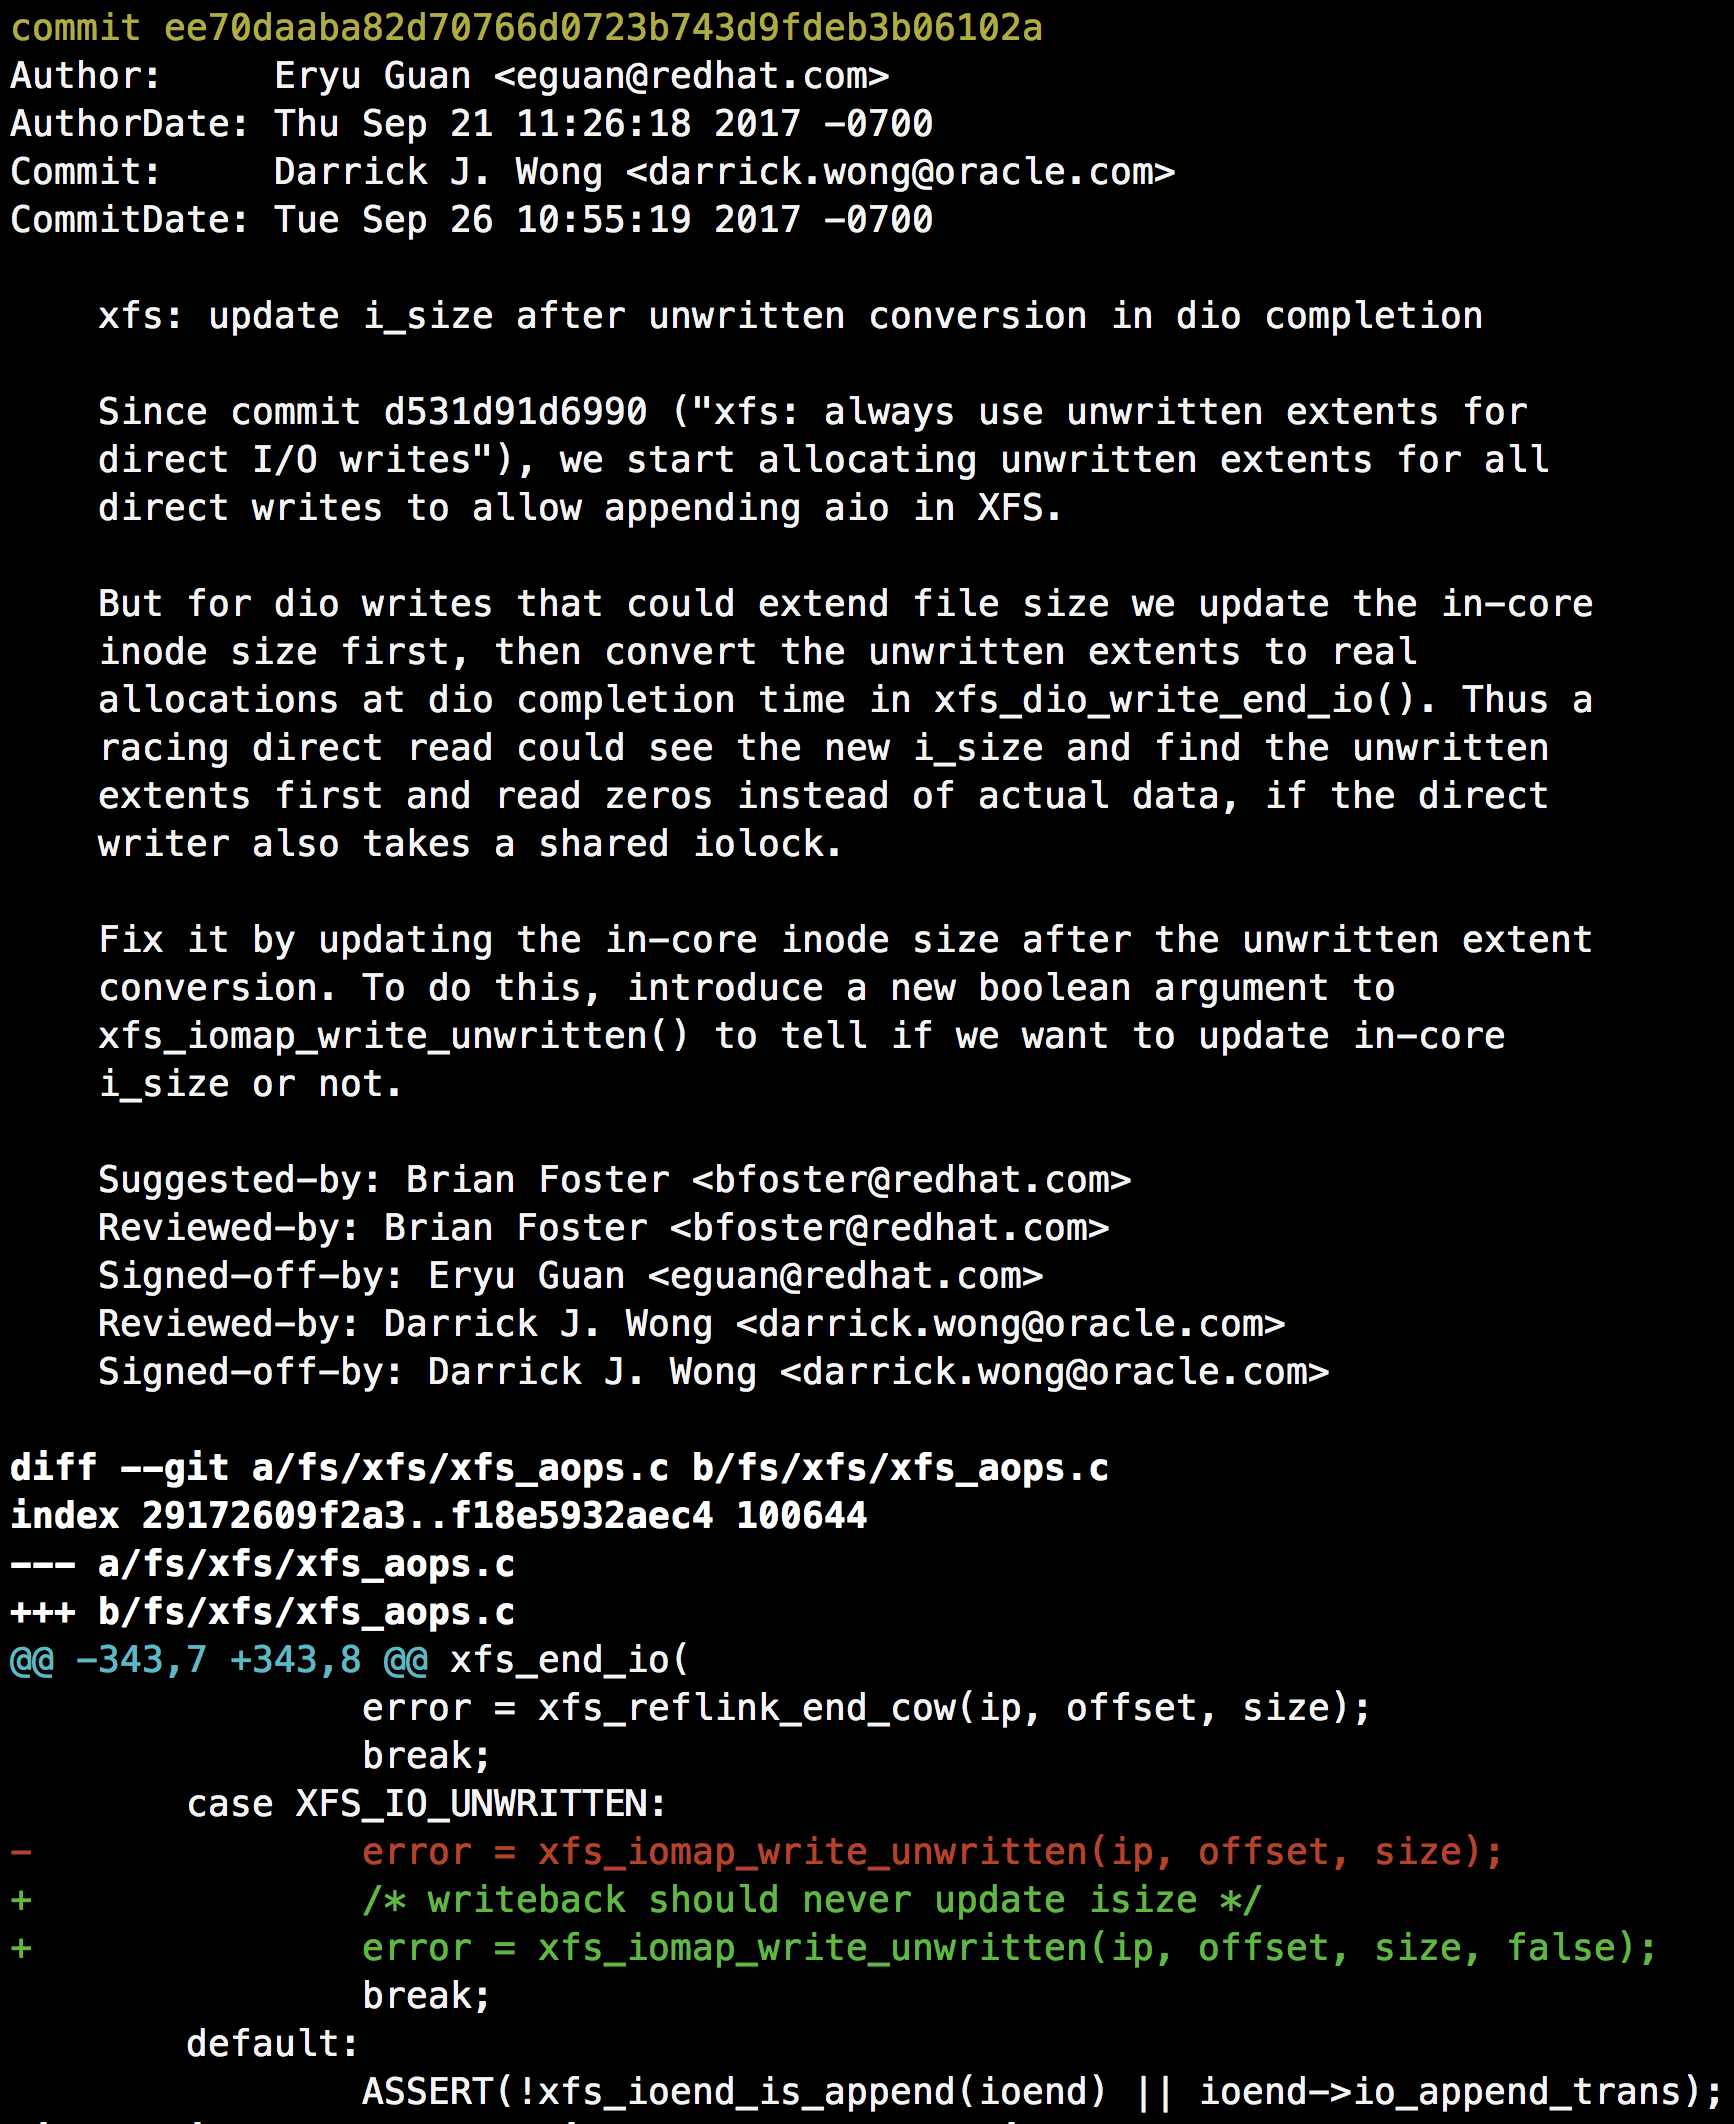
\includegraphics[width=3.5in]{commit_anatomy}
\caption{The anatomy of a commit}
\label{fig:commit_anatomy}
\end{figure}

\begin{itemize}
	\item \textbf{Commit ID:} The "name" of the commit.
	\item \textbf{Commit Author:} Name and email address of the developer who \textit{wrote}, or \textit{authored} the code change.
	\item \textbf{Author Date:} Time, date, and timezone at which the changes were submitted.
	\item \textbf{Commit Committer:} Name and email address of the person who committed the code to the repository.
	\item \textbf{Commit Date:} Time, date, and timezone at which the commit was committed tot he repository.
\end{itemize}

In the scope of the Linux Kernel, the Commit Author rarely the Commit Committer. As explained in \autoref{sec:contrib-process}, the author is the person who wrote the code, and then submitted it for review as a patch in an email. The commit committer is the person that recieved, accepted, and commited the changes to their repository.

The commit message contains the following datapoints:

\begin{itemize}
	\item \textbf{Commit summary:} Often called the commit title, a brief explaination of the purpose of the commit. 
	\item \textbf{Commit Message:} In depth explaination of the purpose of the commit.
	\item \textbf{Credit Attribution Tags:} List of people who were involved in the commit and the nature of their involvment. 
\end{itemize}

There are many different types of credit atribution tags, each describing the way the person contributed to the commit. The most common ones, and the ones we use in this study are: \textit{Signed-off-by}, \textit{Reviewed-by}, and \textit{Acked-by} (acknoledged by). According to \alex{cite https://www.kernel.org/doc/html/v4.12/process/submitting-patches.html} the tags have the following meanings. \textit{Signed-off-by} indicates the developer assisted in the creation of the patch or that she committed it upstream. \textit{Acked-by} is used by developers who were not involved in the creation of the patch but wanted to record their approval. \textit{Reviewed-by} is used to credit developers who contributed reviews to the submitted patch. 

The commit diff, which sits at the end of the git log output, shows the exact files and lines that were modified by the author of the commit. Git uses the commit diffs to apply the changes to the files in the repository. The diff can be percieved as the set of instructions to transform the source code into the desired state.




\subsection{The Linux Contribution Process}
\label{sec:contrib-process}  


Altough Linux uses Git as its version control system, most developer cannot commit directly to the repository. In fact, the developers and maintainers use several different repositories in the development process. The main repository (also called the main tree, of the main line) is maintained by Linus Torvald, the creator of Linux. For a developer to have their code changes integrated into an official release of the Linux Kernel, their changes must be submitted and accepted by Linus Torvalds, as he has the last word on any code being added to the main tree. 

Submitting code changes \textit{upstream}, means to submit changes hoping they will be \textit{merged} into the main tree, and thus into an official Linux release. To achieve this, there is a set of guidelines to follow, as the Linux Kernel follows a strict development cadence and has high code quality standards. First, the code submitted must follow the Linux coding style \alex{cite coding style https://01.org/linuxgraphics/gfx-docs/drm/process/coding-style.html}. It is important to impose a strict coding style in projects of the scale of the linux kernel. Code comming from tens of thousands of developers would become very hard to maintain is everyone cubmitted code with their own coding style. 

Secondly, developers must follow the submission process guidelines. In the vast majority of cases, developers submit their changes to a maintainer. A maintainer is in charge of maintaining a specifi subsystem. A subsystem can be represented as a series of files that work together to serve a certain purpose. When a developer is unsure of who to send the changes to, they can consult the \texttt{MAINTAINERS} file, or use the script \texttt{get\_maintainer.pl} to discover persone responsible for a certain file. The developer must send her changes in the form of a patch the modified subsystem's mailing list. 

Naturally, maintainers must review the patches to ensure that they are worthy of being integrated into their subsytem tree. These reviews usally occur in the email thread following the email patch. The patch author will probably have to improve their code changes according to the maintainer's reviews. If maintainers are satisfied with a patch, they will \textit{commit} it to their repository. As explained in \autoref{sec:commit_anatomy}, for each commit, git differenciates between the \textbf{commit author} and the \textbf{commit committer}. 

Before submitting changes to Linus, maintainers usually send the changes acquired in their repository to \textit{linux-next}\footnote{\url{https://01.org/linuxgraphics/gfx-docs/drm/process/howto.html\#becoming-a-kernel-developer}}. They may do so through an email as a patch, although submitting large changes is easier throught Git. Linux-next is where the integration testing occurs. This is where developers and maintainers make sure new code changes do not interfere with the rest of the code base and do not introduce any bugs. Linus will pull commits that have been in the -next tree for a few weeks \alex{cite: https://01.org/linuxgraphics/gfx-docs/drm/process/howto.html\#becoming-a-kernel-developer}. Linux-next ensures important bugs introduced by new commits are discovered and dealt with before being committed to the main tree, as these bugs would drastically slow down the release cycle. 


The main tree uses a specific releace cycle. After a new version is releases, 4.13 for instance, the \textit{merge window} opens for release 4.14. This two-week long merge window is the only opportunity to submit new code changes in hope to have them integrated in release 4.14. Linus pulls most of the changes from linux-next during that time period because these changes are les likely to cause bugs and thus delay the next release. After two weeks, the merge window closes and linux 4.14-rc1 is released. Then, developers work on ensuring that the kernel is as stable as possible. For approximately 6 to 8 weeks, linus will only accept patches that address bugs introduced by commits merged during the merge window. The only exception is new drivers. New drivers can be submitted outside of the merge window because bugs introduced by drivers are self contained, and only affect users using the specific driver. A new -rc comes out about every week, until Linus declares that the kernel is stable enough to be released. 

Furthermore, large subsytems impose their own release schedule to developers. For instance, the Net subsystem also has two main trees: \texttt{net} and \texttt{net-next}. Net-next recieves all changes submitted to the net subsystem. Once the linus' merge window opens, net-next closes, and all the changes accumulated over the last 10 weeks will be submitted to the main tree. At this point, the net tree will recieve all the fixed related to commits that were committed to the main tree. Once Linus' merge window closes, net-next reopens and developers are free to submit new patches again. 

As stated above, the contribution process relies heavily on emails. The reason why the linux community does not use tools such as github or gerrit is that those tools would not scale to the size of the linux community \citep{armstrong}. And even though the email-based system has been very reliable over the lifetime of the project, there is one drawback. Once a patch is committed to the subsytem tree, and after the commit makes its way upstream to the main tree, there is no easy way to recover the discussion that took place in the mailing list. We address this issue by leveraging an existing algorithm that was introduced and evaluated in \citep{msr13jojo} and \citep{jiang14}. We scaled the algorithm and made the output data available to linux developers.

The process described in this section shows the number of different activities in which Linux developers participate. Previous models, which based their measure of expertise on number of lines of code and commits, do not account for some of the activities undertaken by Linux experts. We build an expertise model which considers a widder aray of metric to assess developer expertise. Since the Linux contribution process is similar to the one used by other organizations, this model could be accurate in other large software projects. 

% \footnote{\url{https://01.org/linuxgraphics/gfx-docs/drm/process/howto.html#becoming-a-kernel-developer}}
% \footnote{\url{https://www.kernel.org/doc/Documentation/networking/netdev-FAQ.txt}}

% linux pulling from linux next: https://www.kernel.org/doc/man-pages/linux-next.html

% linux stable: https://01.org/linuxgraphics/gfx-docs/drm/process/howto.html#x-y-stable-kernel-tree

\section{Hypothesis of Thesis}

Our main research objective is to create a model capable of detecting experts in a certain code area. \autoref{sec:expertise_models} describes previous expertise models created over the years. Our evalution, provided in chapter5, indicates that previous models are not well suited for the linux community. Thus, We based our model on a series of new metrics, which were acquired through different techniques. We were able to make some of these metrics available to the community through two open source projects, which are described in Chapter 3.


\textbf{Hypothesis:} Expertise models targeting large software engineering organizations require a look at all development activities, including code reviews and upstream committing.



To explore this hypothesis, we evaluate the relevance of the different activities present in large scale software development for the purpose of measuring expertise. We build an expertise model based on metrics quantifying these activities. Moreover, we include a hirtorical dimention to the model to represent the impact of long term involvement with the software project. Finally, we provide an evaluation of the different activities by comparing the expert recommendations to the data listed in the \texttt{MAINTAINERS} file.






\section{Plan of the Thesis}


The structure of this thesis is as follows. We conduct a litterature review in chapter 2, where we describe previous expertise models and other topics of interest. Chapter 3 gives a detailed overview of the general workflow of the thesis. Chapter 4 gives an indepth look at Email2git, one of the opensourcve project we created. Finally, chapter 5 includes the article we submitted to the  International Conference on Software Analysis, Evolution and Reengineering (SANER).



% Un URL: \href{http://www.polymtl.ca}{École Polytechnique de Montréal}.

% \subsubsection{Une sous-sous-section}
% Les besoins des flots de données peuvent être catégorisés selon
% quatre paramètres importants \citep[voir][sect.\,5.4]{Tanenbaum} ou:
% \begin{itemize}
% %%
% %% ELEMENTS DE LA PROBLEMATIQUE
% %%
% \section{Éléments de la problématique}  % environ 3 pages
% La description de \mbox{l'en-tête} commun de RSVP est détaillée ci-dessous:\\
% \begin{tabular}{p{1in}p{4.5in}}
% &\\ % Ligne vide
% \texttt{Ver}: & \texttt{4 bits}\\
%           & Version du protocole. La version actuelle est~1.\\[5pt]
% \texttt{Flags}: & \texttt{4 bits}\\
%           & Aucun Flag n'est défini. L'émetteur doit (\textbf{MUST})
%           mettre le champ à zéro et le récepteur doit (\textbf{MUST})
%           ignorer ce champ.\\[5pt]
% \texttt{Msg Type}: & \texttt{8 bits}\\
%           & Type de message\\[5pt]
% \texttt{Checksum}: & \texttt{16 bits}\\
%           & Complément à un du complément à un de la somme des champs
%           de \mbox{l'en-tête}, avec le champ Checksum à~0 pour des
%           fins de calcul. La valeur~0 signifie qu'aucun Checksum n'a
%           été transmis. Si le résultat du calcul du Checksum donne~0,
%           la valeur 0xFFFF doit être stockée dans ce champ.\\[5pt]
% \texttt{TTL}: & \texttt{8 bits}\\
%           & Valeur originelle du champ \texttt{TTL} utilisée pour
%           transmettre ce message.\\[5pt]
% \texttt{Reserved}: & \texttt{8 bits}\\
%           & Réservé pour usage futur. L'émetteur doit (\textbf{MUST})
%           mettre le champ à zéro et le récepteur doit (\textbf{MUST})
%           ignorer ce champ.\\[5pt]
% \texttt{Length}: & \texttt{16 bits}\\
%           & Longueur totale du message en octets, incluant
%           \mbox{l'en-tête} commun et tous les objets de longueur
%           variable.
% \end{tabular}

% \subsection{Autres types de structures de données}
% L'énumération:
% \begin{enumerate}
% \item Un item~;
% \item Un autre item.
% \end{enumerate}


% \subsection{Le protocole IPv6}
% Voir la Figure~\ref{fig:IPv6} pour plus de détails. Le champs DSCP est
% décrit dans le Tableau~\ref{tab:RangesDSCP}.

% \begin{figure}[htb]
% \centering
% 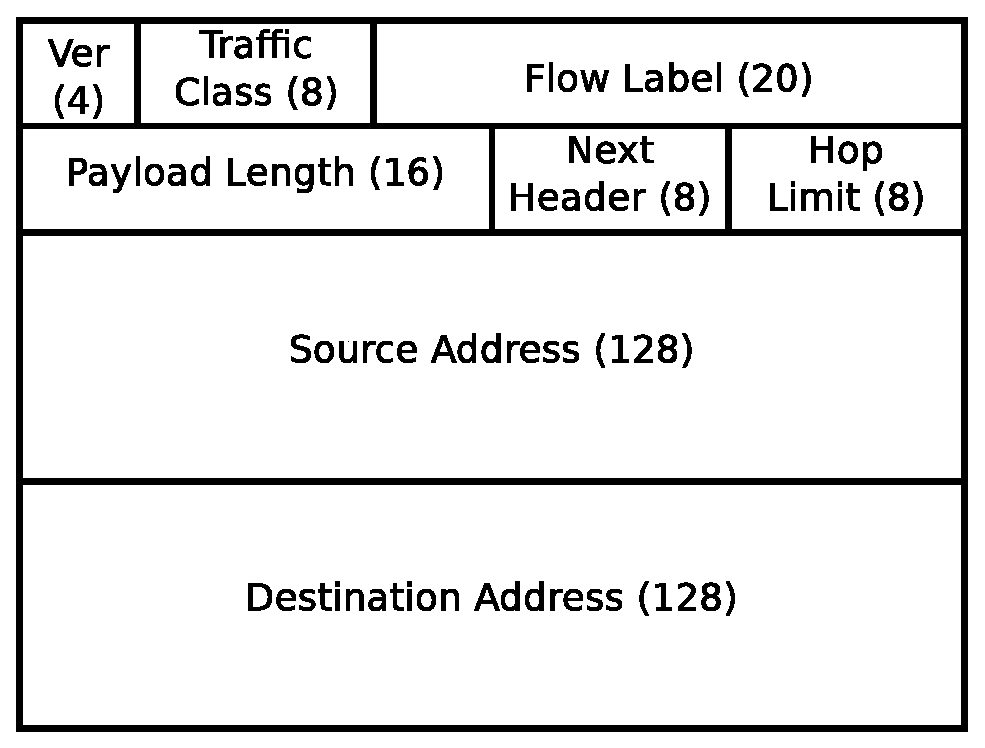
\includegraphics[width=4in]{IPv6_header}
% \caption{L'en-tête IPv6}
% \label{fig:IPv6}
% \end{figure}

% \begin{table}[ht]
% \caption{Plages de valeurs pour le champ \texttt{DSCP}}
% \centering
% \begin{tabular}{|c|c|l|}
% \hline\rowcolor[gray]{0.8}\color{black}
% Plage & Valeurs & Règle d'assignation\\\hline
% 1 & xxxxx0 & Assignation par une norme de l'IANA\\\hline
% 2 & xxxx11 & Expérimentation/Usage local\\\hline
% 3 & xxxx01 & Expérimentation/Usage local (pourrait être jointe à la plage 1)\\\hline
% \end{tabular}
% \label{tab:RangesDSCP}
% \end{table}

% % On veut éviter que la figure et le tableau soient placés au-delà de la section courante.
% \FloatBarrier


% %%
% %% OBJECTIFS DE RECHERCHE
% %%
% \section{Objectifs de recherche}  % 0.5 page
% Les objectifs de la recherche sont de concevoir un algorithme $O(n)$.


% %%
% %% PLAN DU MEMOIRE
% %%
% \section{Plan du mémoire}  % 0.5 page
% Un tableau:
% \begin{table}[htbp]
%   \centering
%   \caption{Constantes et variables du modèle analytique}
%   \begin{tabular}{|c|l|}
%     \hline\rowcolor[gray]{0.8}\color{black}
%     Symbole         & Description\\\hline
%     $\lambda$       & Taux d'arrivée moyen des requêtes de réservation de ressources\\\hline
%     $\frac{1}{\mu}$ & Durée moyenne d'une session\\\hline
%     $C$             & Capacité d'une cellule (nombre de sessions supportées)\\\hline
%     $v_{moy}$       & Vitesse moyenne des MN dans le réseau d'accès\\\hline
%     $L$             & Longueur d'un côté d'une cellule carrée\\\hline
%     $n$             & Nombre moyen de MN dans une cellule\\\hline
%     $\rho$          & Charge d'une cellule\\\hline
%     $P_b$           & Probabilité de blocage d'une requête de réservation\\\hline
%     $P_f$           & Probabilité d'interruption forcée d'une session\\\hline
%     $P_c$           & Probabilité de compléter une session avec succès\\\hline
%     $\Delta{}T$     & Délai de transmission\\\hline
%   \end{tabular}
%   \label{tab:Definitions}
% \end{table}

% La formule d'\mbox{Erlang-B}:
% \begin{equation}
%   P_b = \frac{\frac{\rho^C}{C!}}{\sum\limits_{x=0}^{C}\frac{\rho^x}{x!}}
%   \label{eq:Pblock}
% \end{equation}

% Une autre équation:
% \begin{equation}
%   \begin{split}
%     P_c &= (1 - P_b) \times (1 -  P_f)^N\\
%         &= (1 - P_b)^{N+1}
%   \end{split}
%   \label{eq:ProbComplete}
% \end{equation}

% Enfin, l'expression suivante indique le moment à partir duquel les
% réservations de ressources sont en place:
% \begin{equation}
%   \Delta{}T_{init} =
%   \begin{cases}
%     2\Delta{}T_{E2E} & \Delta{}T_{wan} > (\Delta{}T_{rad} + \Delta{}T_{net})\\
%     \Delta{}T_{E2E} + 3(\Delta{}T_{rad} + \Delta{}T_{net}) & \text{sinon}
%   \end{cases}
%   \label{eq:InitCost}
% \end{equation}

% \paragraph{Le taux de paquets perdus} correspond au nombre de paquets
% éliminés à cause d'une erreur de \emph{checksum} à un n\oe{}ud
% quelconque ou d'une situation de congestion. Le taux de paquets perdus
% pour un chemin est déterminé de la façon suivante:
% \begin{equation}
%   \label{eq:genPLR}
%   PLR_P = 1 - \prod_{i=1}^N(1 - PLR_i)
% \end{equation}

% Toutefois, si les taux d'erreurs sont très faibles, comme c'est
% généralement le cas pour des liens optiques, on peut approximer
% $PLR_P$ de façon à le transformer en un paramètre additif:
% \begin{equation}
%   \label{eq:approxPLR}
%   \begin{split}
%     PLR_{L_1 \oplus L_2} &= 1 - (1 - PLR_1)(1 - PLR_2)\\
%     &= 1 - (1 - PLR_2 - PLR_1 + \underbrace{PLR_1
%       \times PLR_2}_\text{négligeable})\qquad PLR_1 \ll 1,
%     PLR_2 \ll 1\\
%     &\approx PLR_1 + PLR_2
%   \end{split}
% \end{equation}



% Une courbe:
% \begin{figure}[htb]
% \centering
% 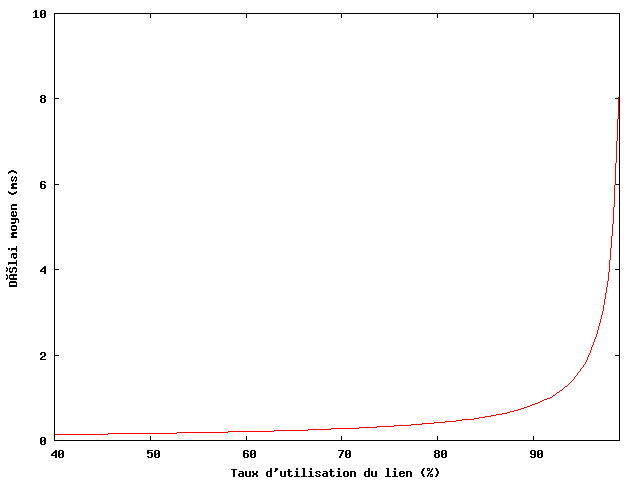
\includegraphics[width=5in]{LinkUsage}
% \caption{Délai moyen en fonction du taux d'utilisation d'un lien}
% \label{fig:LinkUse}
% \end{figure}

% \selectlanguage{english}
% This paragraph is formatted by \LaTeX{} according to the standard rules of the
% English language (\mbox{e.g.} hyphenation).
% \selectlanguage{french}

% L'arithmétique en virgule flottante peut entraîner des erreurs
% d'approximation et il est important d'en être conscient
% \citep[voir][]{Goldberg1991}.

% De même, les calculs effectués sur une carte graphique (GPU) peuvent
% introduire des erreurs d'approximation \citep{Benz2012, DSilva2012,
%   Dabrowski2011, DeDinechin2011, DeFigueiredo2004, Filliatre2007,
%   Fousse2007, Goubault2001, Goubault2008, Harder, Higham2002, Tanenbaum,
%   Whitehead2011, mpmath, nichols2010, nvidia2012, Benz2012, Bao2013}.
       % Introduction au sujet de recherche.
\Chapter{CRITICAL LITERATURE REVIEW}\label{sec:RevLitt}


Our research project touches upon two areas of software engineering research: \textit{mining software repositories} and \textit{software engineering expertise}. Besides these two research fields, we relied on another type of literature to conduct this research project: Git and Linux documentation. This chapter provides a critical literature review of the our two academic research areas and a description of the information available in the Linux and Git documentation, as well as how it helped us finding solutions for the problems encoutered.



\section{Mining Software Repositories}

In addition to providing a contribution platform, \ac{SCM} systems track and save large amounts of information about each changes brought to the source code. During the lifetime of the project, the \ac{SCM} acquires a large amount of data about the development of the project. Mining software repositories researchers \textit{mine} this data for their research projects. 

Software repositories are not limited to \ac{SCM}. There are other entities present in software repositories that research mine to gather information about software projects. These entities include bug tracking systems, mailing lists, source code, and issue tracking systems. Over the years, researchers have used mining software reporistories techniques that enabled them to research different topics of software engineering~\citep{Bird-2009}.

In the scope of our research, we used mining software repositories techniques in each different part of the project. Chapter 3 discusses two open source projects we created during this research project. The data used for both projects came from mining the Linux Kernel repository. We eventually used this data for the creation of our expertise model.

One of the difficulty often encountered by researchers in mining software repositories is the inability to link data coming from different entities of the software repository. In the case of the linux kernel, the dificulty was to link data from the mailing lists to the data from the git repository. A dificulty we addressed with an algorithm in \citep{jiang14}. 

Furthermore, \citep{armstrong} studied the difference between \textit{unicast} and \textit{broadcast} review systems. A unicast review system, like gerrit, provides an environment in which the code reviews are only visible by the author of the patch. On the contrary, broadcast review system, like the email system used by the Linux community, shows the code reviews to each reader of the mailing list. There are advantages and inconvinients to both systems. The authors note that unicast reviews lead to less bugs in the future, but that broadcast systems allows for faster review cycles and allow beginers to learn the code base faster. 



\section{Software Engineering Expertise}
\label{sec:expertise_models}

Many different studies explored the concept of expertise in software engineering. the authors of two early studies, Expertise Browser \citep{mockus02} and Expertise Recommender\citep{McDonald}, expressed the importance of understanding developers' expertise level. McDonald et al. approach the topic from a problem solving percpective. Today's developers have many different resources at their disposal for the purpose of problem solving. Stack Overflow\footnote{\url{https://stackoverflow.com/}}, a programming question answer exchange, is used by developers from around the world that are lookiing for solutions for complex problems. Before Stack Overflow's creation in 2008, developers did not have easy access to a large database of solutions provided by \textit{experts} from various topics. The authors of the Expertise Recommender were seeking to solve this problem by providing an architecture capable of recommending experts for given parts of the software project, for the sake of finding an expert to solve an issue. \citep{mockus02} approach the issue differently. They provide and expertise model to solve the issue of replacing or adding new expert to a distributed software engineering project. They argue that the tool would reduce the time lost by engineers attempting to find a new expert for their team. 


Each of these previous studies ~\citep{Bhattacharya}, ~\citep{mockus02}, ~\citep{McDonald}, and~\citep{Fritz-2007} base their measures of expertise among developers on the tacit assumption that experience is acquired through development activities, such as number of lines of code contributes or the number of commits authored. The author in \citep{Fritz-2007} examined the reliability of this assumption. Through a review of the many studies in psychology on knowledge and expertise, \citep{Fritz-2007} disovered that there was no sufficient evidence that activity does determine one's knowledge. The authors conducted a quantitative study on 19 java programmer to assess the accuracy of these finding. With this survey, they discovered that multiple activity related heuristics influenced developers' knowledge. These heurstics include authorship, role, work experience, and activity, which confirms the suitablility of the metrics used in previous work (LOC and commits). Furthermore,~\citep{Fritz-2007} mention the effect of code stability to code knolwedge. The authors emphasized the importance of the notion of history in determining knowledge.  

Globally, we found that the previous expertise models on the topic fail to address several important activities present in software development mentioned in~\citep{Fritz-2007}.Even though the authors give insightful advice on how developers acquire knoledge, they do not provide an expertise model capable of recommending expert for a certain code area. 


\section{Open Source Participation}

Previous work studies developers' motivation in \ac{OSS}. In~\citep{Wu-oss}, warn that the losely organized nature of OSS development could be associated with a high turnover rate and in unexpected departures. Other work ~\citep{Rigby} studies the impact of a high turn over on the organization. The authors argue that departing developers bring the amount of knowledge they acquired during their time as a contributor. We believe that this implies that OSS projects are at risk of knoledge loss and we believe that accurate expertise modeling could assist in addressing this issue.





  % Revue de littérature.
\Chapter{RESEARCH GENERAL WORKFLOW}\label{sec:Theme1}



My master research consisted of two different parallel projects. The first project consisted in a collaboration with the Linux Foundation and the second consisted of a case study of expertise evolution in the Linux Kernel.






Two sides of the project:

\begin{itemize}
\item open source tools	
  \begin{itemize}
	\item srcmap
	\item email2git
	\item integrating email2git with cregit
	\item traveling to conferences, talking to linux devs/maintainers, introducing the tools and getting feedback
	\item How email2git can help us with out research 
  \end{itemize}	
\item Reseach paper 
\end{itemize}             % Premier thème (Doctorat) ou "Détails de la Solution" (Maîtrise).
\Chapter{EMAIL2GIT: FROM ACADEMIC RESEARCH TO OPEN-SOURCE SOFTWARE}\label{sec:Theme2}

As explained in \autoref{sec:Introduction}, the linux contribution process is a strong email-based system that has proven to be reliable and scalable over the years. Like in many other organizations, the linux development community makes extensive use of code reviews to ensure the quality of contributors' code submissions. These code reviews occur in the mailing lists, where the patch was first introduced. After accepting and integrating the patch to the git repository, it is usually very hard to recover the original patch, the code reviews, and the discussion that took place during the code reviews. 

Other tools have addressed this issue by providing a code review environment and by keeping track of the code review for each commit. However, these environments often do not broadcast the code reviews to everyone. These \textit{unicast} review environment only allow the author to read the code reviews. In a quantitative study, \citep{armstrong} examined the differences between \textit{unicast} and \textit{broadcast} review system. The authors discovered that broadcast allows for faster review cycle, and provides learning material for new developers. The linux community never used these tool for upstream contributions as they would not scale to the size of the linux community. 


To address the lack of way to backtrack reviews, we implemented Email2git. The tool is able to find, for a given linux commit, the orignal patches and the code reviews. This chapter introduce Email2git, from its inception, to its deployement to production. 

\section{Previous Publications and Original Algorithm}

The original algorithm capable of backtracking patches from commits was introduced in two papers~\citep{msr13jojo,jiang14} published by Jiang, a former member of the MCIS Lab. The general idea of the algorithm was to compare the +/- lines from both the git commits and the email patches. A match was found if the proportion of identical +/- lines was above a certain threshold. Although this script was a great proof of concept, it had difficulties scalling to 8 years of emails and commits. 

For example, there are 5 +/- lines in a commit $A$'s diff. The algorithm iterates through the patches present in the dataset, comparing the 5 +/- lines form the commit to the +/- lines from each patch. To compare the +/- lines from the commits and the patches, the algorithm find the proportion of identical lines in both the commit and the patch. A patch will be matched to commit $A$ if the proportion of identical lines is above a certain threshold. 

\section{Scalling the Algorithm}

Since we had access to email patches dating back to 2009, we decided to extract git commits from the Linux git repository from the same date until the release of linux v4.11, which represent over \textit{500,000 commits} to analyse. Unfortunatly, this amount of data was too large for the orignal algorithm to parse in a timely fashion.

Which called for a new, scalable algorithm that leverages heuristics mentioned in \citep{msr13jojo,jiang14}.

We were able to separate the matching process into multiple different phases. After each phase, the matched commits and patches are removed from the dataset to reduce the workload for the next phase. The different phases are explained in this section. 

\subsection{Patch Email Subject}

The most important heuristic that drastically increased the matching speed is the \textit{email subject - commit summary} concept. The built-in git features \texttt{git format-patch} and \texttt{git send-email} allows developers to easily submit their changes to a maintainer by email according to the Linux Kernel Contribution guidelines\footnote{\url{https://kernelnewbies.org/FirstKernelPatch}}. This or these emails contain all the meta-data that will eventually be included in the commit, if the patch is accepted. The meta-data includes metrics such as: time sent, author, commit message, ... If the patch is accepted, the maintainer can use another git command to integrate the patch into her repository: \texttt{git am}\footnote{\url{https://git-scm.com/docs/git-am}}. This command will automatically exctract the patch info and keep the relevant information in the commit. The piece of information we are interested in is the email subject. \texttt{Git am} automatically saves the email subject and uses it the "commit summary". This commit summary, or commit title, is the first line of the commit message as explained in \autoref{sec:commit_anatomy}. Comparing both strings of characters allows for a very quick first phase of matching.



\subsection{Author and Affected Files}

Even though the number of commits was reduced by half after the first phase, I was unable to make the old script fast enough to parse the rest of the data in a timely fashion. Thus, I had to find a way to use the available meta-data to speed up the matching. The first data point I used was the \textit{author name}. As depicted in \autoref{fig:author_matching}, one can use the name and email address of the \textit{commit author} to pin point to the patches that were sent by the same person. In other words, to find a match for each commit, the algorithm has to parse a handfull of patches instead of hundreds of thousand. Similarly, the name of the files affected by a commit and a patch can drasticaly help the performance of the +/- line algorithm. Through some regular expression and text parsing, we can retrieve the files that are modified in the patch and the \textit{commit diff}. Since the author-based matching is slighty faster and returns more matches than the file-based matching, we start with the former, removing each matched commit and patch to reduce the workload of the next phase.

\begin{figure}[htb]
\centering
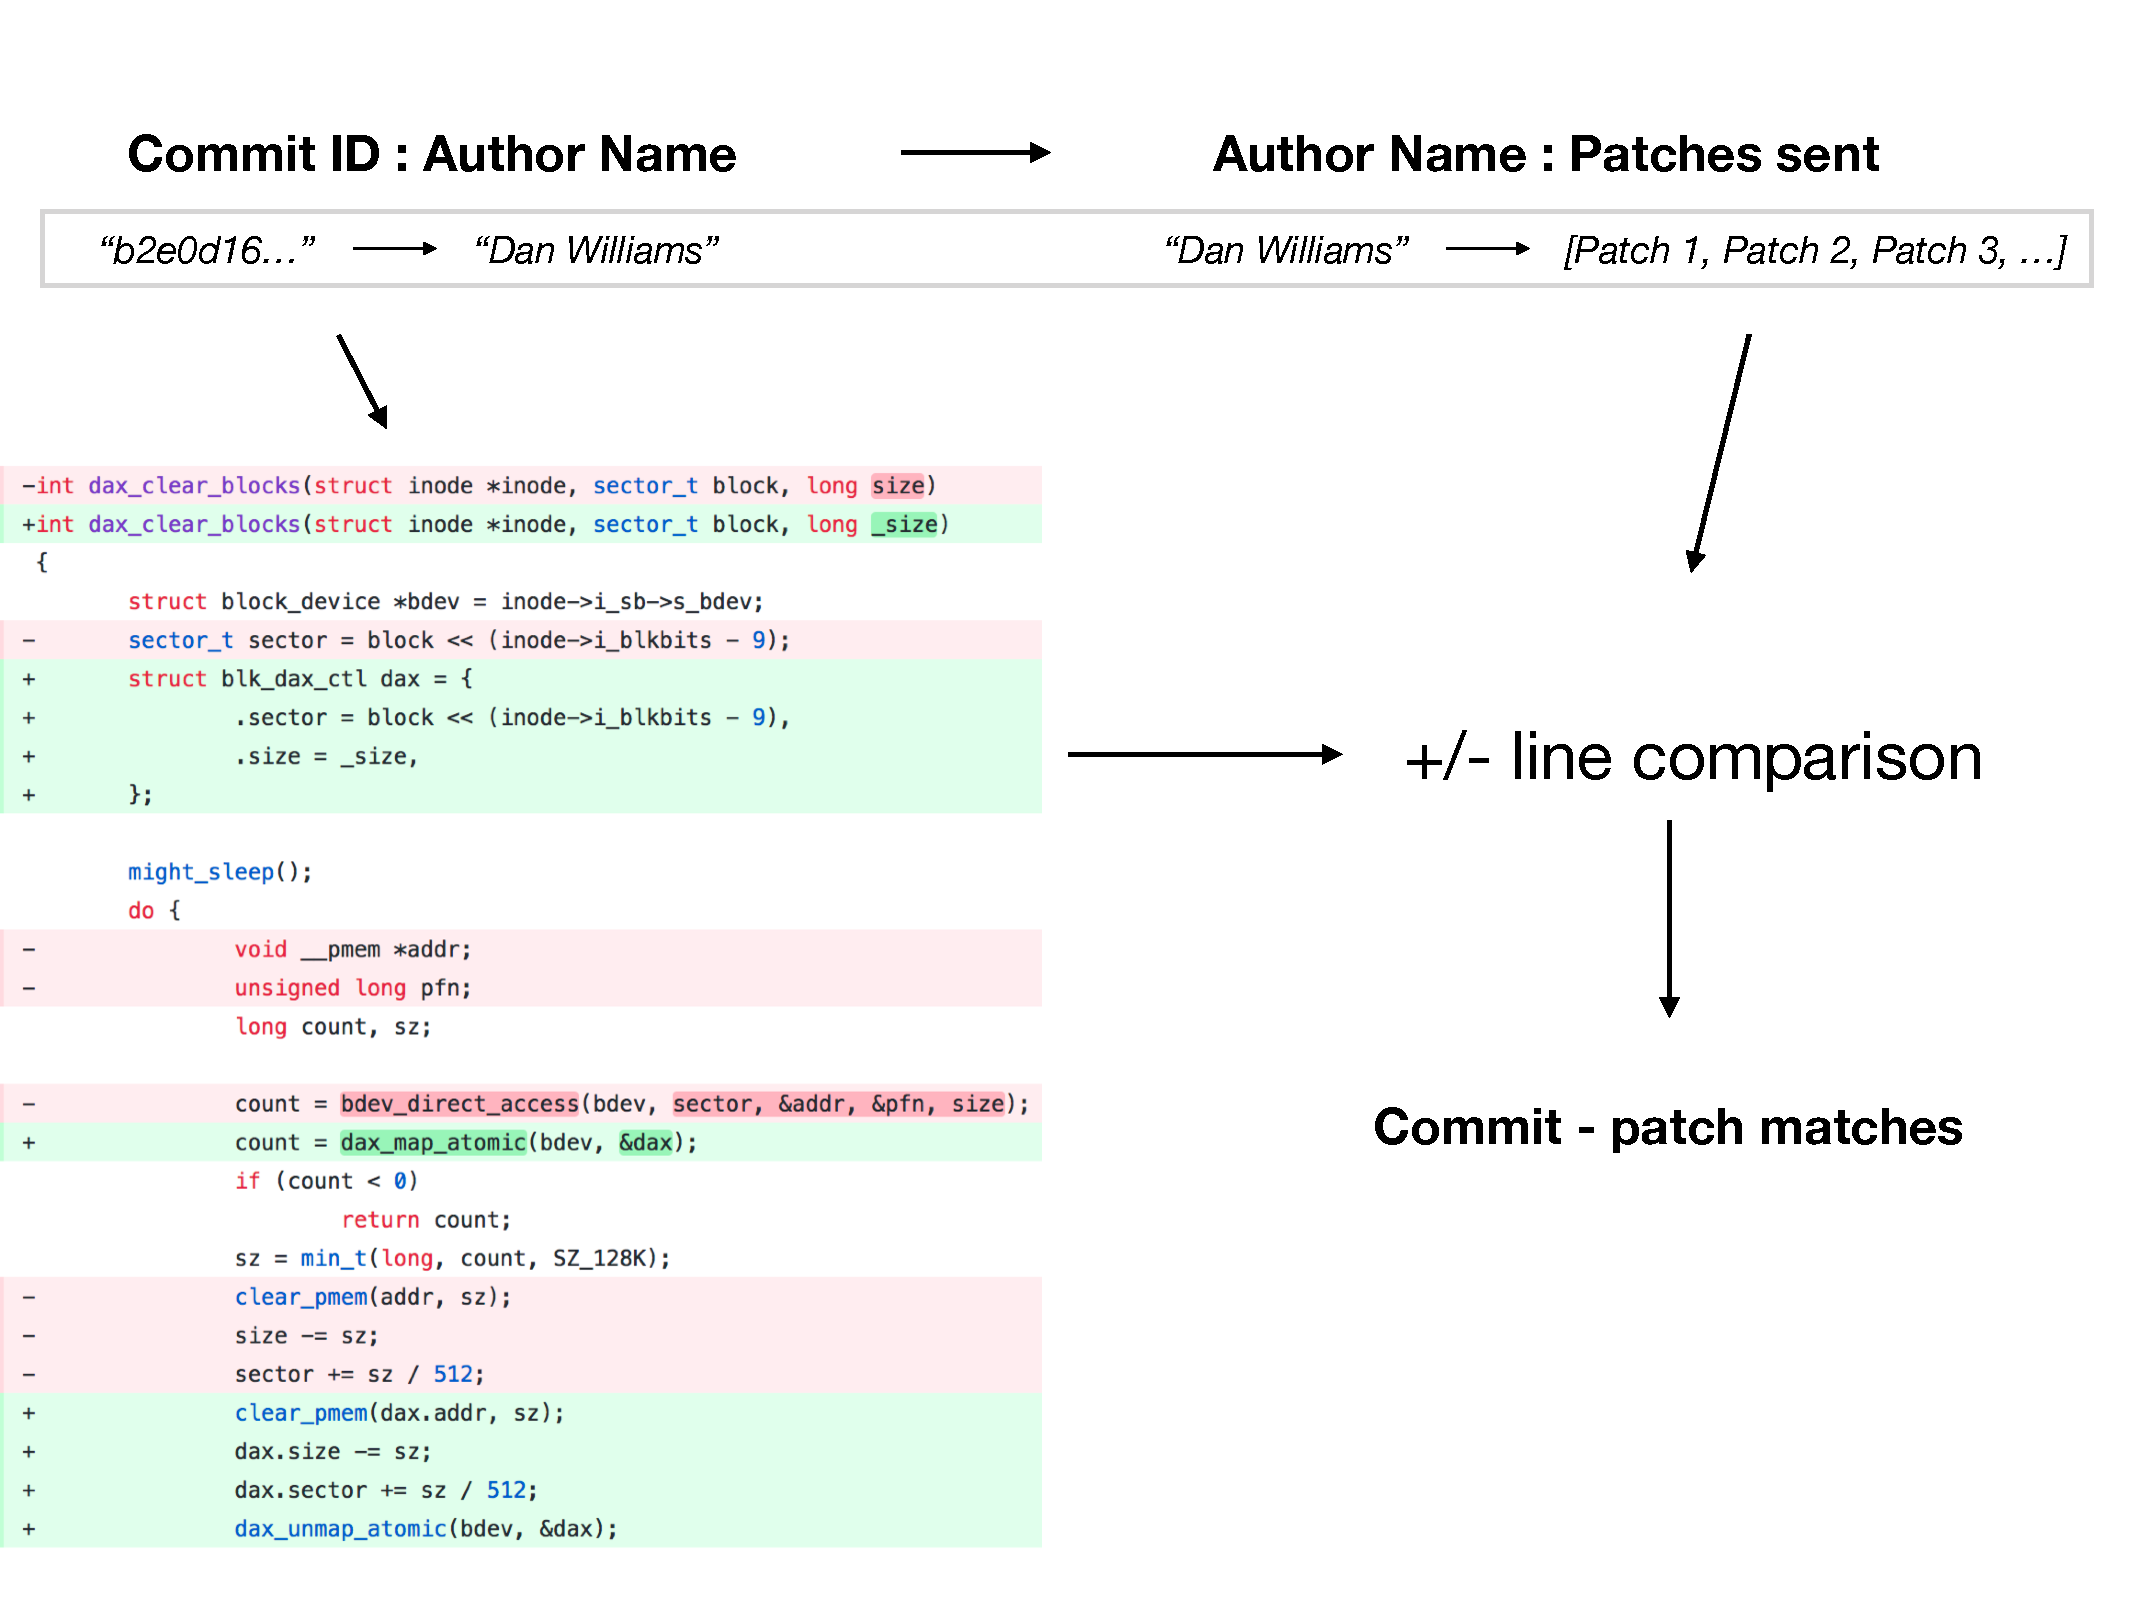
\includegraphics[width=5in]{author_matching_tmp}
\caption{Using the patch sender to assist matching}
\label{fig:author_matching}
\end{figure}


\section{The Data}

There are two sides to this matching process: the Linux git repository and the archives containing the patches sent in mailing lists over the years. We need to extract the diff (+/- lines), the metadata, and the subject and commit summary from both side. The scripts used for each part of the data extraction are available on the Email2git project's github under the GPL-3.0 license \footnote{\url{https://github.com/alexcourouble/email2git}}.

Because we wanted Email2git to be a usable and practical tool, we needed a way to display the patches and the code reviews in a browser. Fortunatly, an existing open-source tool called \textbf{Patchwork}\footnote{\url{https://github.com/getpatchwork/patchwork}} perfectly answers our requirements. Patchwork is a tool designed to assist maintainers of open source projects using an email-based contribution process. It tracks the mailing lists used by developers to submit patches and recieve code reviews. The tool extracts each detected patch as well as its associated reviews, then displays them in a web-based user interface. Additionally, Patchwork stores the patches in a database, along side a unique ID that can be used to generate a URL to that patch.

We were granted read access to the MySQL database behind a patchwork instance hosted on kernel.org\footnote{\url{https://patchwork.kernel.org/}}. This instance has been tracking 69 of the many linux subsystems mailing lists since 2009, giving us the oportunity to analyse over \textit{1.4 million} patches.

In addition to being a data source, patchwork.kernel.org also represents a way for us to display the patches and the code reviews associated with commits to the users. The only limitation of this patchwork instance is that it does not track some major mailing lists, particularly some of the \texttt{Net} mailing lists.


\subsection{The Commits}

First, we need to extract the commit summary from each commit after 2009. This date is our lower bound because our email data from patchwork.kernel.org only has email patches dating back to 2009. The commit summary is the first line of the commit message, which makes it very easy to retrieve. The script \texttt{subject\_data\_gen/commit\_subject\_generator.py} reads a git log output and stores the commit summary for each commit in a SQLite3 database. The exact git log command used is the following:
\begin{lstlisting}
git log --no-merges --pretty=format:"%H,%ct,%s" --after={2009-01-01}
\end{lstlisting}
The \texttt{pretty} option formats the output according to the passed parameters. 

The next step on this side of the data is to extract the data for the other phases of the matching process. The script \texttt{lines\_data\_prep/git\_prep.py} is more complicated, as there is more data to parse and save. This script reads the authors and the files affected by each commit. It will then create two maps: commit ID to author, and commit ID to files affected. These maps, which exist as python dictionaries are then saved to two separate pickle files\footnote{\url{https://docs.python.org/2/library/pickle.html}}, which make writting, reading, and storing data a fast and easy. This script also extracts the +/- lines from the commit diff and stores them in a pickle file as well. 



\subsection{The Patches}

The patches are stored on a remote serve in a MySQL database, the same database that hosts the patchwork.kernel.org data. Through the help of SQL queries, I dumped all the necessary data in csv files to avoid complications arising from handling a production database. Once those csv files created, I could parse them with the help of two python scripts available in the Email2git githubg repository. \texttt{subject\_data\_gen/patchwork/pwSubjectFull.py} takes care of the subject data and \texttt{lines\_data\_prep/pw\_prep.py} takes care of the authors, file names, and +/- lines of the patches. Here again, the subject data is stored in a SQLite3 database, and the line data is stored in pickle files. 









\section{Integrating Email2git with Cregit}

Cregit is a project that aim at providing a finer grain approach to \textit{git blame}. The blame option in git returns the name of the developer who last changed a line of code in the source code. It provides a great way to quickly unmask the developers responsible for code in the Source Code. However, it has a serious limitation: git blame assigns a line to a developer even after a small modification to that line. For instance, if developer $A$ writes \texttt{print "Hello world"}, this line will then become associated with developer $A$. However, if developer $B$ modifies the line to read \texttt{print "Hello world!"}, git blame will associate the line with devloper $B$ even though developer $B$ only added a character. 

Cregit addresses this limitation by tokenizing the source code in a git repository to enables git blame at a token level, instead of a line level. This provides a better understanding of the true authors of the source code. A tokensize version of the Linux kernel source code is available online through the cregit interface\footnote{\url{https://cregit.linuxsources.org/}}.

\begin{figure}[htb]
\centering
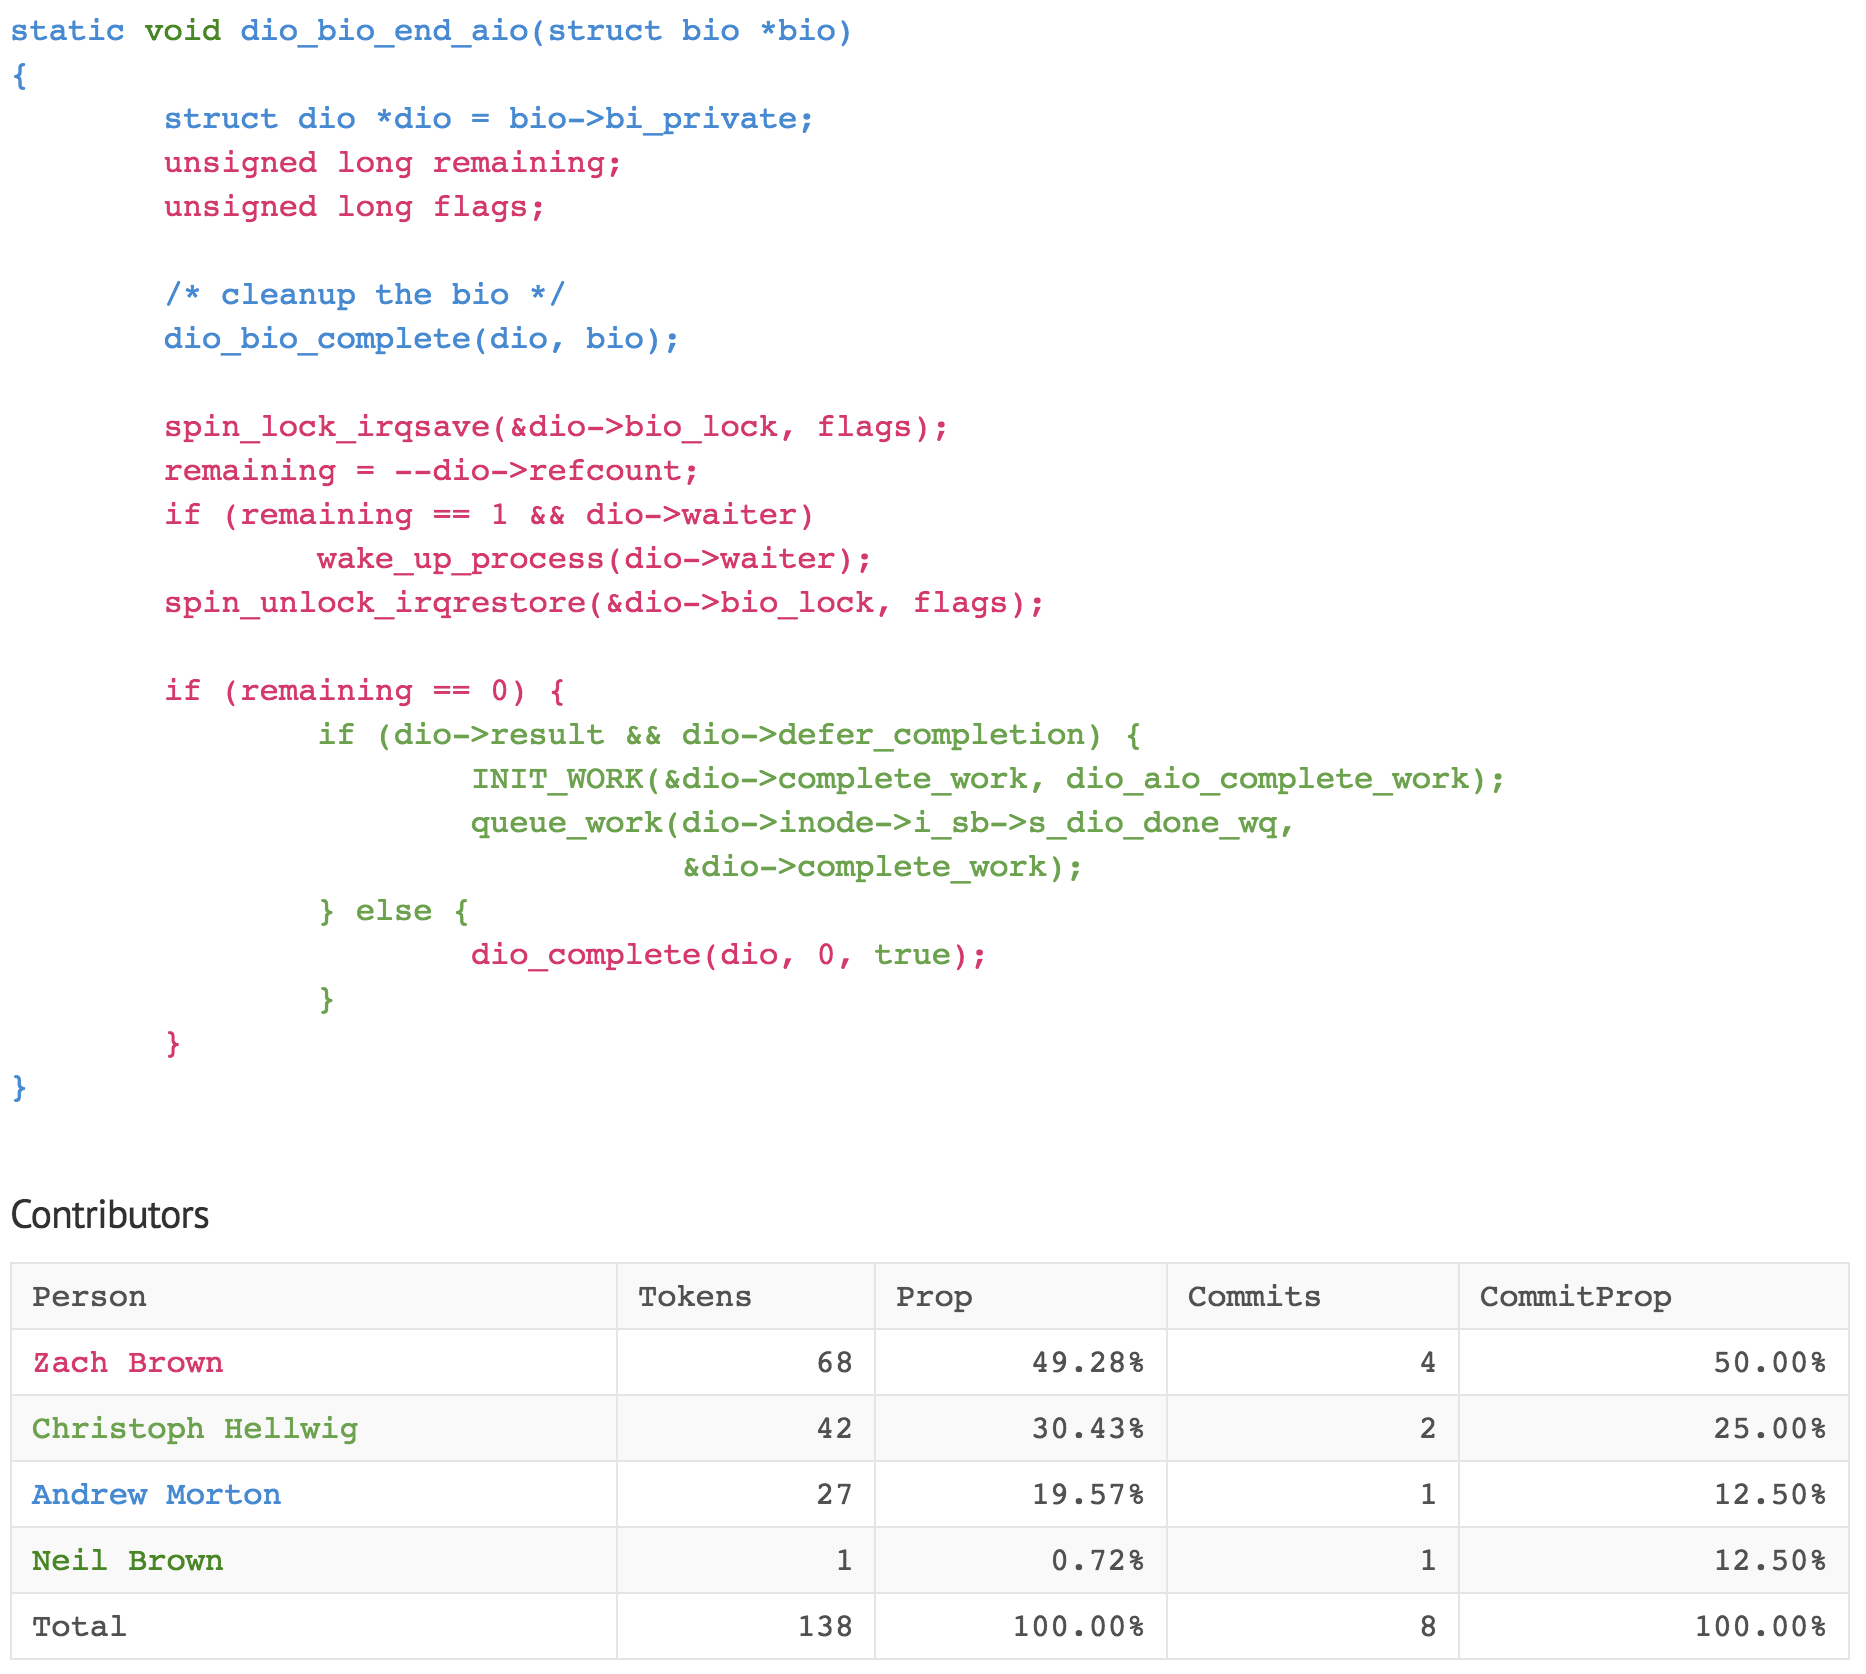
\includegraphics[width=3.5in]{cregit_code}
\caption{Tokenized source code as it appears on Cregit.}
\label{fig:cregit_code}
\end{figure}

\autoref{fig:cregit_code} shows tokenized linux code as it appears on the Cregit interface. In an effort to ease the access to email2git data, we decided to provide access to the matches through cregit. To this end, I modified the user interface to display a window containing all the available patches after clicking on a token, as shown in \autoref{fig:cregit_matches}. 

\begin{figure}[htb]
\centering
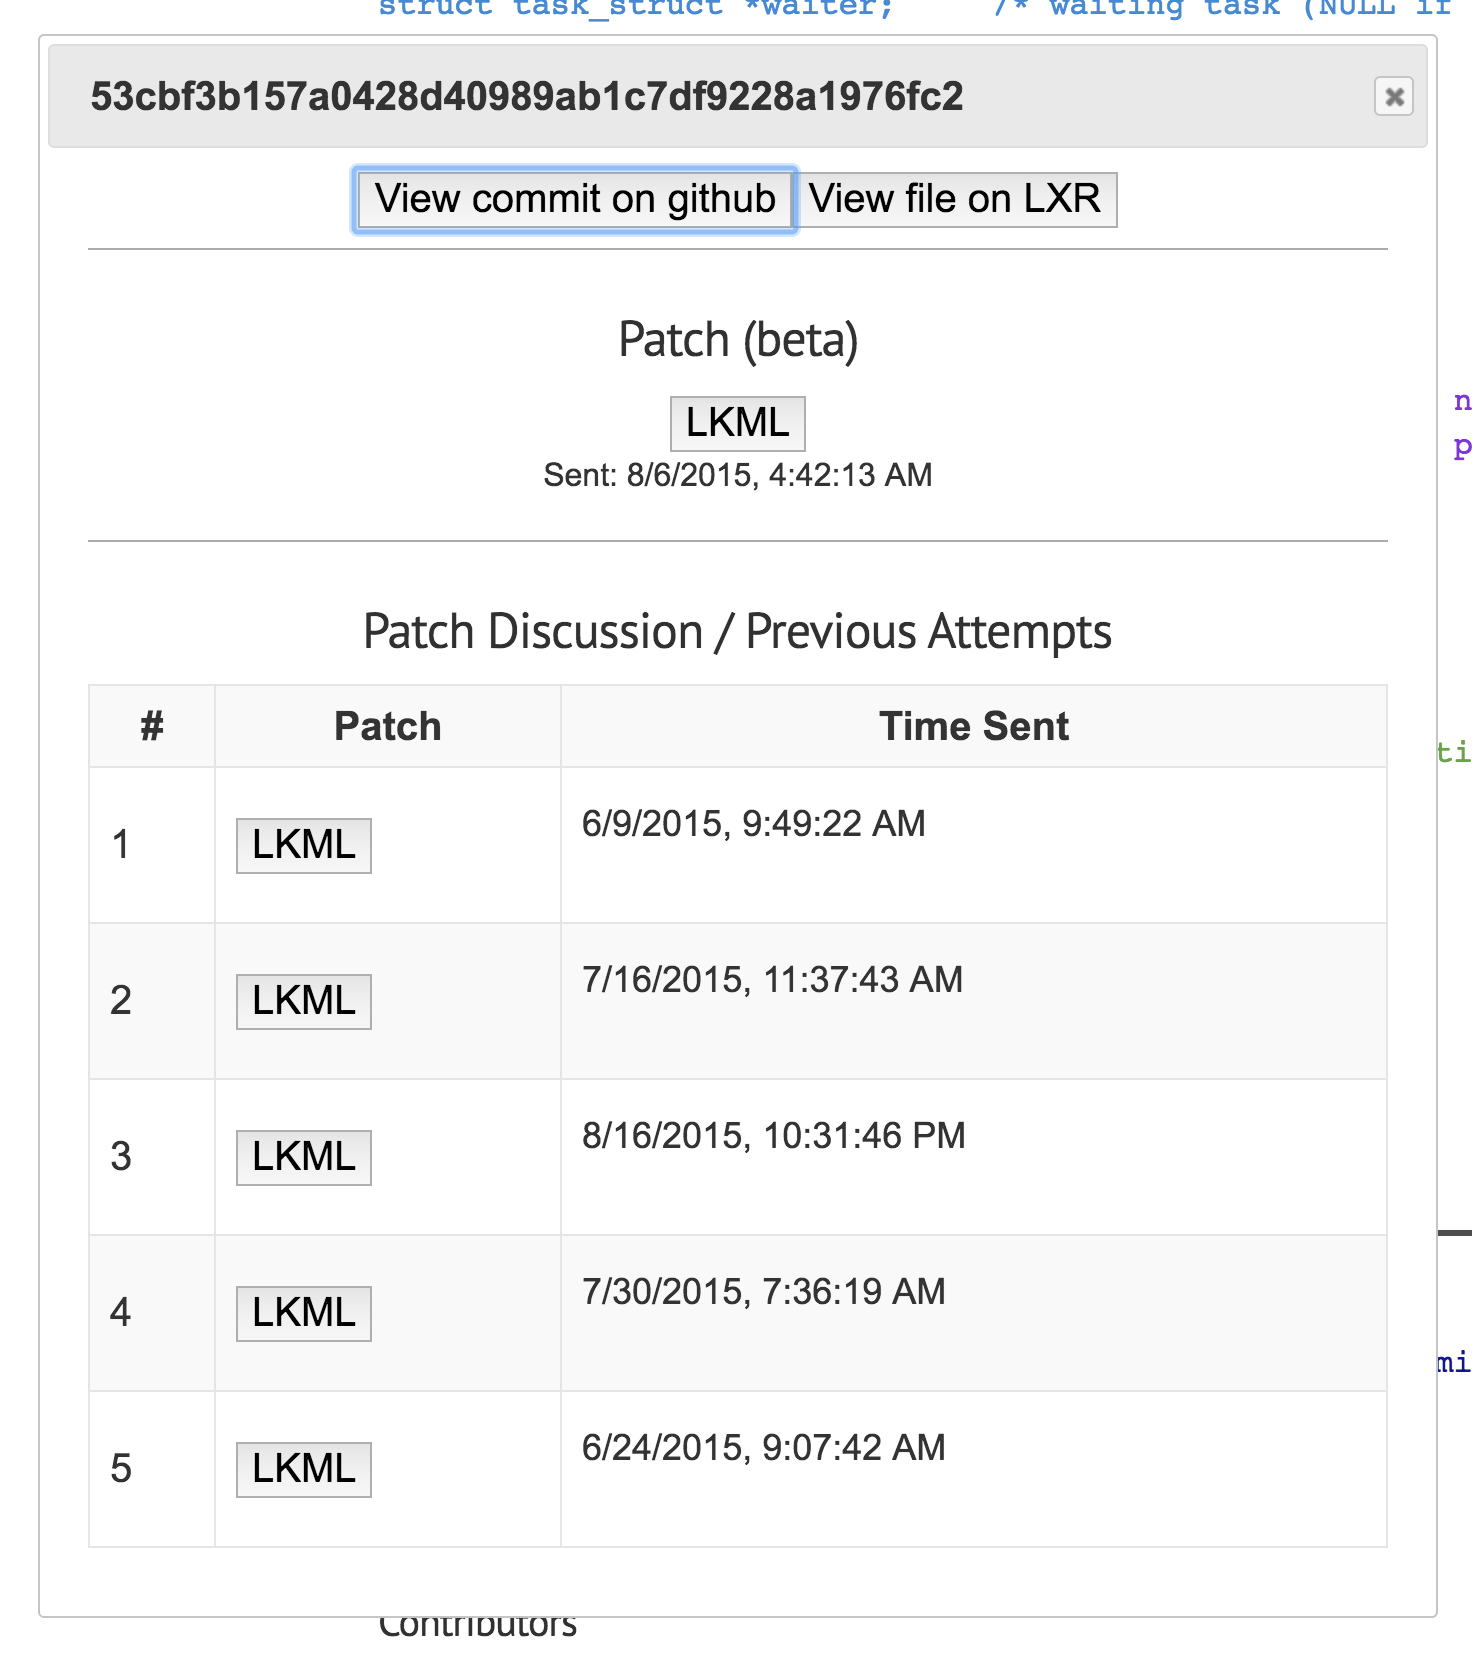
\includegraphics[width=3.5in]{cregit_matches}
\caption{Window containing the patches that introduced the commit associated with the clicked token}
\label{fig:cregit_matches}
\end{figure}




\section{Providing Access to the Matches}

Email2git's original inteded contribution was to increase the amount of information existing around a commit by providing access to the conversation that took place during the creation of the patch. And now that matches have been generated and saved, we need a way to make the information available to linux developers. Each match is composed of four elements: the \textit{commit ID}, the \textit{patchwork permalink ID}, the \textit{date}, and the \textit{phase} that found the match (subject, author, or file). The patchwork permalink ID is used to point to the patch and conversation on patchwork.kernel.org.

As discussed in the previous section, the matches are available through two platforms: cregit and as a standalone commit lookup page. And although both platforms use the same UI and fetching mechanism to display the links to patchwork, the user experience is fundamentally different. On cregit, users navigate the interface by browsing the tokenized files. Once the user clicks on a token, we display a window containing the links to the patches and converstation that introduced that token to the source code. Note that in this case, the user need not to know the commit ID of of the token of interest. The commit ID, which is necessary to retrieve the patches, is hard-coded in the html element containing the token. The HTML element containing a token looks like this:

\begin{lstlisting}[language=HTML]
<a onclick="return 
windowpopLinux('2ebda74fd6c9d3fc3b9f0234fc519795e23025a5')">
	include
</a>
\end{lstlisting}

The onclick event calls a function defined in a global javascript file: \texttt{cregit.js}. In the original implementation of the cregit interface, this function would open a new browser window and show the commit associated by the token on github. So I modifed \texttt{cregit.js} to disable the "popup mechanism" and to instead use the commit ID to fetch the patchwork permalinks IDs from the server. The matches are stored as csv files named after the commit ID they are associated with on the server hosting the interface. The assyncronous requested is done throught Papaparse\footnote{\url{http://papaparse.com/}}, a powerful opensource javascript library capable of downloading and parsing csv files from the client. The javascript code that generate the URLs from the permalinks and displays the new window lives in a callback function that executes after the request is complete. We were able to keep the "view commit on github" feature, by showing a button in the new window.  

On the standalone commit ID lookup page, the mechanism is almost identical, but the user experience is completely different. Instead of clicking on a token, the user knows the commit ID in advance, as they might have encountered it while trying to fix a bug, or read a \texttt{git log} output. The user copies and pastes the commit ID in the search bar, and the match window appears with a list of dated links to patchwork. The lookup page verifies whether the commit ID is a SHA-1 hash with the following regex:

\begin{lstlisting}
// removing white space
cid = cid.replace(/\s/g, '');

// validating input
if (!/\b[0-9a-f]{40,40}\b/.test(cid)){
    window.alert("The input should be a full 40-character SHA1 hash.");
    return;
}
\end{lstlisting}





\section{Introducing Email2git to the Opensource Community}

We undertook various efforts to make our work more visible to the linux and open source community in general. The first effort was a blog post published on linux.com\footnote{\url{https://www.linux.com/blog/email2git-matching-linux-code-its-mailing-list-discussions}}. This blog post discusses email2git and its integration with cregit. This blog post was shared on Facebook and Twiter by the Linux Foundation and by other developers, which helped spreading the word about our work. In addition to this blogpost, I gave a refereed talk at the Open Source Summit and the Linux Plumbers Conference in Los Angeles. This gave me the oportunity to give a demo, explain the underlying algorithm and finally discuss the project with developer and recieve crucial feedback. An article\footnote{\url{https://lwn.net/Articles/734018/}} was published on LWN.net by Jake Edge following my talk. It explained the algorithm, the chalenges faced, and mentioned some of the questions that were asked during the talk.


The linux developers feedback included the following points:
\begin{enumerate}
	\item \textbf{Including patch zero.} The patch zero is the email that introduces a multi-patch series. A multi-patch series is a large set of changes that is split over multiple emails. The patch zero contains information regarding the entirety of the patch series. Our current source of matches, lkml.kernel.org, uses patchwork 1.0, which did not track the patch zero. The patch zero feature was implemented in Patchwork 2.0.

	\item \textbf{Tracking Linux-next.} As mentioned in \autoref{sec:Introduction}, linux-next is the branch used for integration testing. Developers would benefit from review discussions to help fix bugs that arised from integrating commits to linux-next. 

	\item \textbf{Give credit to reviewers.} The \texttt{reviewed-by} tag is used to give credit to the developers that contributed during a patch review. However, some reviewers often do not receive the credit they deserve after contributing in reviews. Our tool could automate the \texttt{reviewed-by} tags.

	\item \textbf{Guidelines for more accurate matching.} A developer suggested the creation of a list of guidelines for developers to follow in their development process. These guidelines would promote the use of the built-in git features that use the email subject as commit-summary. If addopted by the community, those guidelines would increase the proportion of matches found. 
\end{enumerate}


\section{Evaluation}

To evaluate the current state of the tool, we look at the number of commits Email2git was able to match. Overall, the algorithm matched 57\% of the non-merge commits since 2009. We look at the proportion of commits matched in the largest subdirectories of the Linux Kernel source code. \autoref{fig:matched_proportions} presents these proportions. The proportion of matches found is uneveny spread accross the different subdirectories of the Linux Kernel source code. For example, the \texttt{kernel} and \texttt{mm} directories have about \textbf{70\%} of their commits matched. On the other hand, the \texttt{net} directory only has \textbf{25\%} of their commits matched. This is mainly due to the absence of key mailing list from our email dataset. One of these mailing lists is \texttt{netdev}, where many patches related to net development are sent. This is reflected in the low proportion of commits matched in the \texttt{net} subdirectory. 


\begin{figure}[htb]
\centering
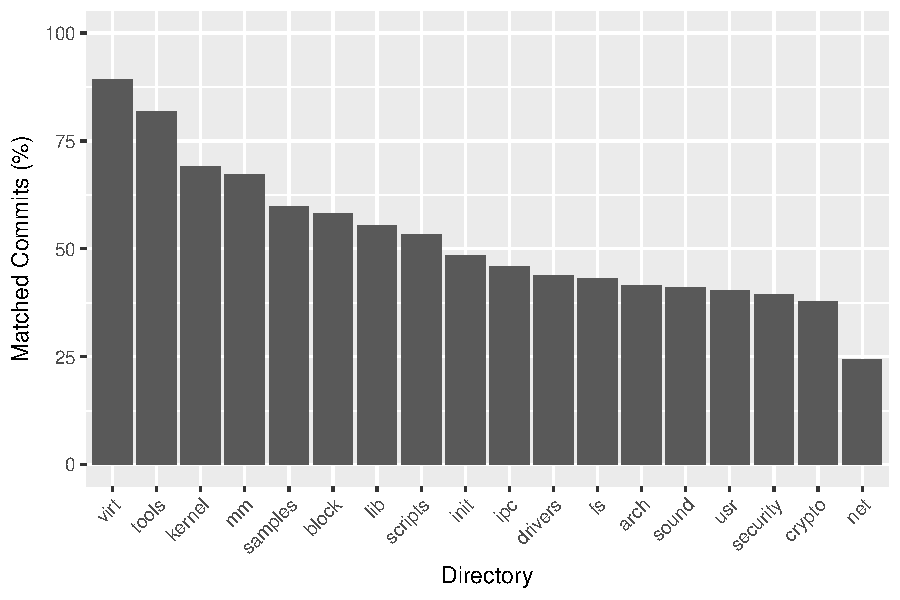
\includegraphics[width=5in]{plots/matched_commits_dir}
\caption{Percentage of matched commits in Linux subdirectories, from 2009 to the time of writing this thesis}
\label{fig:matched_proportions}
\end{figure}

Furthermore, we can break down the matches by the stage of the algorithm that generated them. The first phase of the algorithm, which uses the email subject, finds about \textbf{95\%} of the final set of matches. The second part of the algorithm, which uses the author and filename based matching, finds \textbf{5\%} of the final matches. It is important to note that the second phase of the algorithm is exposed to less commits than the first phase. The commits matched by the first phase are removed from the dataset before starting the second phase. This implies that the second phase will inherently find less matches than the first phase. We tested the performance of the line-based algorithm (both author and filename) on a subset of commit and patches to understand its performance. The algorithm found a \textit{correct} match for \textit{26\%} of the analysed commits.



Finally, we are running an analytics script on the server hosting the matches to understand the usage of the data and to know the proportion of requested commit IDs are not matched. Removing the whitespace and assuring the validity of the string ensures the accuracy of these statistics, by recuding the number of failed requests due to a poorly formated commit ID.

\begin{figure}[htb]
\centering
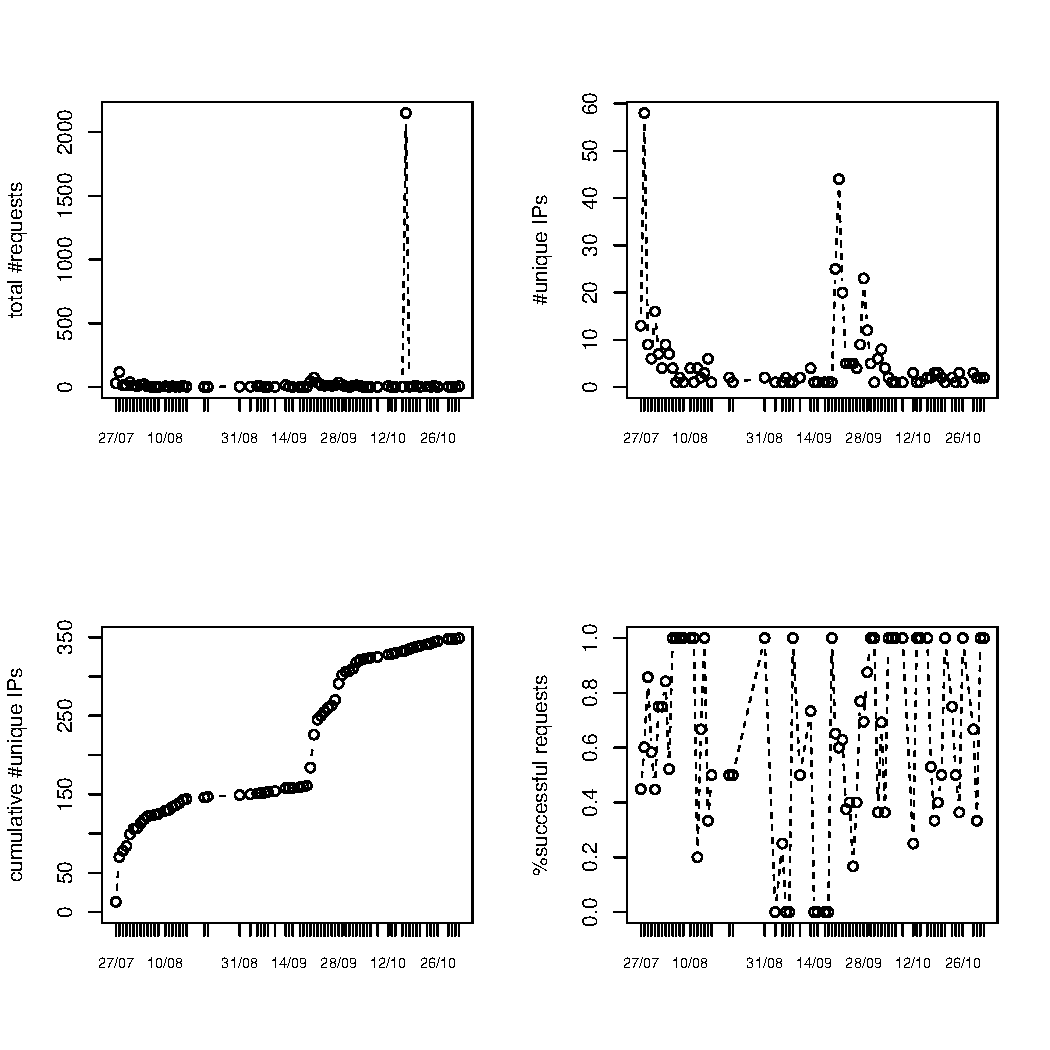
\includegraphics[width=5in]{analytics}
\caption{Plots created from the analytic}
\label{fig:analytics}
\end{figure}

\autoref{fig:analytics} displays the plots created by the analytics script running on the server. We observe two peaks in number of unique IP addresses at two different moments: at the end of July and in mid September. The former date corresponds to the day we introduced Email2git in a blogpost on linux.com and the latter corresponds to the talk I gave at the Open Source Summit North America in Los Angeles. 

\section{Conclusion}

We leveraged the lessons learned from Srcmap while creating Email2git. The purpose of Email2git was to answer a complain coming from multiple developers and maintainers: the difficulty of finding an email discussion about patches that were eventually integratted in the Linux Kernel. Understanding the Linux community allowed us to better introduce our tool when we released it, as explained in Chapter 4. Moreover, the data acquired in the implementation of Email2git served as one of the metrics used by our expertise model as explained in chapter 5.


\alex{email2git successful, developers showed interest, }

\alex{intention to pursue development, features to implement. patchwork with more mailing lists. Pipeline. linux next}
             % Second thème (Doctorat) ou "Résultats théoriques et expérimentaux" (Maîtrise).
\Chapter{ARTICLE 1: ON HISTORY-AWARE MULTI-ACTIVITY EXPERTISE MODELS}\label{sec:Theme3}

\section{Abstract}

As software evolves, a maintainer's contributions will gradually vanish as they are being replaced by other developers' code, slowly eroding the maintainer's footprint in the software project. Even though this maintainer's knowledge of the file did not disappear overnight, to outsiders, the maintainer and her expertise have become invisible. Through an empirical study on 5 years of Linux development history, this paper analyses this phenomenon of expertise erosion by building a 2-dimensional model of maintainer expertise involving a range of maintainer activities and involving activity data on more than one release. Using these models, we found that although many Linux maintainers' own coding footprint has regressed over time, their expertise is perpetuated through involvement in other development activities such as patch reviews and committing upstream on behalf of other developers. Considering such activities over time further improves recommendation models.


\section{Introduction}

As reported by Damien et al.~\cite{turnover}, employee turnover is a major challenge of information technology organizations. Estimations of the cost of losing an employee amount to between 0.5 and 1.5 times her salary, with the cost of replacing a software engineer in particular exceeding \$100,000~\cite{economist5988}. These costs are not limited to the software engineer's company, but also spread to open source development. In their 2017 Linux kernel report, Corbet et al.~\cite{corbet17} noted that ``well over 85 percent of all kernel development is demonstrably done by developers who are being paid for their work''. In fact, only 8.2\% of all kernel commits were made by volunteer developers. Hence, developer turn-over in companies risks to impact open source development as well!



Apart from improving the working conditions and onboarding procedures, software organizations (both closed and open source) need to invest time in finding the ``right'' expert to replace a parting maintainer. While it is possible to train newcomers and bring them up to speed (e.g., one third of the kernel contributors in the last 12 months were newcomers, and 60\% of those made their contribution as employee), the term ``right'' refers to having a similar profile, allowing the new maintainer to seamlessly fit in and continue his or her predecessor's work, without significant loss of knowledge. Thanks to the widespread adoption of agile development and open source development models, software development has become a collaborative endeavor, in which knowledge is shared across the members of an organization, hence in principle it should be possible to find contributors with similar profiles.

Unfortunately, there is no consensus on how to measure the profile of a developer, and how to determine whether such a profile indicates the developer to be an maintainer. The simplest way to measure someone's development activities is to count the number of code changes (e.g., Git commits) authored. This is for example how Corbet et al. determine the most active developers and organizations in Linux kernel development~\cite{corbet17}. Yet, at the same time, they note that ``The total number of patches signed off by Linus Torvalds (207, or 0.3 percent of the total) continues its long-term decline. That reflects the increasing amount of delegation to subsystem maintainers who do the bulk of the patch review and merging.'' Worse, developer rankings based on the number of commits differed substantially based on the period during which this metric was measured (e.g., ranking based on last 10 years vs. last year). At a minimum, one needs to be careful interpreting these and other measures such as a developer's code legacy as shown by ``git blame''~\cite{Bhattacharya, mockus02, McDonald, Fritz-2007}.
To make developer expertise measures more robust and reliable, this paper proposes a 2-dimensional contribution footprint model, addressing two important issues with current expertise models. First of all, while the amount of code written by a person can be an important indicator of expertise, 
it does not take into consideration the actions of people who do not directly contribute
source code, such as those who review it or discuss it on mailing lists or issue repositories. Our footprint measure combines indicators of multiple kinds of developer activities.

Second, as indicated by Corbet et al., current measures focus on a given software release or development period, basically ignoring the development activities that happened before.
While a person who wrote 50\% of the code changes of the previous release could be less of an expert than a person who
wrote 50\% of the code changes of the current release, the former developer might have been ill or absent, or might have been the one mentoring the latter developer. As such, both developers should be considered as experts, not just the latter developer. Our footprint measure allows to consider a developer's activities across different time periods.

We empirically evaluate the footprint model's ability to detect maintainers on 5 years of Linux kernel development history, addressing the following research questions:



\begin{description}
\item[\textit{RQ1)}] \textit{\rqone }
\end{description}

\begin{myindentpar}{1cm}
Almost 1 out of 4 subsystems has seen a change in maintainership during the last 22 Linux kernel releases, with the code footprint of maintainers gradually decreasing over time.
\end{myindentpar}

\begin{description}
\item[\textit{RQ2)}] \textit{\rqtwo }
\end{description}

\begin{myindentpar}{1cm}
Models involving a maintainers' own code footprint and coordination activities (committing and/or reviewing) perform the best.
\end{myindentpar}

\begin{description}
\item[\textit{RQ3)}] \textit{\rqthree }
\end{description}

\begin{myindentpar}{1cm}
Models considering the last $R$ releases perform better than single-release models.
\end{myindentpar}


\section{Background and Related Work}
\label{sec:backgr-relat-work} 

% Prior work \cite{Wu,Zhou,Ye-icse-2003} discusses developers' motivations to stay an open source project, claiming that developers will likely stop their involvment with the project once their personal goals have been fulfilled. Developers' departure results in knowledge loss \cite{Rigby}, as tacit knowledge about their code will disaprear with them. This knowledge loss associated with developer departure could have a important negative impact if the departing developer happens to be a maintainer. 


Maintainers ensure the longevity of a large open source project like the Linux kernel by not only contributing new code, but also by reviewing and integrating code submitted to their subsystems by other developers. Despite their crucial role in open source development, % maintainers are the backbone of Linux kernel development, yet 
few studies have been done on maintainers~\cite{Zhou-fse}. 
In particular, a maintainer's departure of her subsystem calls for her immediate replacement. However, only a developer with extensive experience in the subsystem can take on the task of maintainer. Hence, in this section, we aim to understand the different expert detection techniques. % \bram{in this paper or in related work section?}.

Software expertise and knowledge have been extensively studied in the past~\cite{Bhattacharya, mockus02, McDonald, Fritz-2007}. Most of this work % regarding software expertise
provides a recommendation system to detect experts among the population of developers. % regarding a particular software project. 
Typically, existing % Most 
recommenders % created in the past
base their assessment of expertise on \textbf{non-historical models}, meaning that they only exploit data of the current snapshot of the software repository, not of earlier versions. These non-historical models use a variety of different metrics to determine expertise.

\textit{Implementation expertise.} This type of metric implies that a developer gains expertise through implementation, in other words, by making changes to a file% ~\cite{Anvik:2007:DIE:1268983.1269018}
, % The earliest models assessed expertise based on changes brought to the source code, which are 
as tracked by a version control system. McDonald~\cite{McDonald} recommends the last developer who made a change to a file as expert for that file, which could be interpreted as file-level \texttt{git blame}. Later, Mockus et al.~\cite{mockus02} improved on the approach proposed by McDonald~\cite{McDonald} by counting the number of changes each developer brought to a file to provide a better expertise recommendation. Girba et al.~\cite{1572315} later improved Mockus et al.'s method~\cite{mockus02} by measuring the size (churn) of each change in terms of lines of code.  %\bram{which is McDonald? be more precise as to how this third paper improves on Mockus}.
% removed bug review paper. It is not relevant enough for us

\textit{Usage Expertise.} Developers gain usage expertise by calling (``using'') specific methods from within their code. This concept of usage expertise was introduced by Schuler and Zimmermann~\cite{Schuler:2008:MUE:1370750.1370779}. In later work~\cite{5306386}, the authors compare the accuracy of usage expertise against implementation expertise recommenders. They concluded that usage expertise recommends experts with similar accuracy to implementation expertise models. 

Additionally, Fritz et al.~\cite{Fritz-2007} validate the accuracy of implementation expertise techniques. After a qualitative study consisting of  19 java developers interviews, they were able to confirm a relationship between changes made (commit frequency) and expertise. In addition to that, they found evidence proving that authorship (as obtained from the amount of churn contributed, or through ``git blame'') is also capable of indicating expertise. In a later study, the authors~\cite{Fritz:2010:DMC:1806799.1806856} create a degree of knowledge model combining both usage and implementation metrics to recommend experts.

% \bram{did these add another kind of expertise metric, or still impl. vs. usage?} 
Bhattacharya et al.~\cite{Bhattacharya} explored the suitability of different implementation expertise metrics depending on a developer's role. They argue that state-of-the-art metrics (lines of code and commits added), being unaware of the developer's role, can lead to inaccurate results. They add that code activity metrics like the number of lines of code added, only describe expertise at a local level and poorly capture global expertise. 


Thus far, all models cited above are not \textbf{history aware}. Hence, they do not take into consideration the effect of time on developer expertise and assume that developers' memory lasts for ever. Based on a survey of psychological literature, Hattori et al.~\cite{Hattori:2012:RCO:2318097.2318145} create a memory retention model to improve expertise models. Memory retention is computed using a Forgetting function, which reduces the weight of older activities to account for memory loss.
%\bram{how? details?} 
The data used in the experiment was acquired by a tool that records information from the developer's IDE. It would be impossible to reproduce this experiment on a project of the scale of the Linux Kernel because it would be impossible to force all Linux developers to use the IDE integrated tool.
%\bram{why? currently no means for reader to understand this important statement}

Although these state-of-the-art techniques are well suited to detect experts among regular developers, who specialize in implementation, they % we believe that they do not properly evaluate more complex expertise, such as that of subsystem maintainers.  
ignore most of the daily tasks of maintainers, such as reviewing and committing code upstream, creating an inherent bias in the expertise models. We address this bias by building expertise models based on a variety of metrics capturing the full breadth of software development activities, and also considering the evolution of such activities over time.




% Ownership.

% Using git blame for finding owner of code \cite{1572315} .
% MSR for accurate authorship \cite{Meng:2013:MSR:2550526.2550579}.







% \begin{itemize}
%   \item explain why experts are important for code quality \cite{Rahman-2011}
% \end{itemize}


% code reviews \cite{Thongtanunam-2016}

% Explain difference between author and commiter \cite{Ihara}

% conclude that current approaches ignore most of the tasks of experts, so need new expertise formula, whiose evaluation is our goal




\section{Measuring Developers' Contribution Footprint}
\label{sec:expertise-formula}

This section discusses the two-dimensional contribution footprint model proposed by this paper to enable identification of experienced team members (e.g., developers, testers, etc.) as candidate maintainers. The first dimension of the footprint model considers a wide range of activities performed by a project member, not only focusing on code changes, but also code review or even a developer's code ``legacy'' (i.e., contributed code that still survives in the code base). The second dimension enhances the first dimension by not only considering the range of activities in the latest release, but \emph{across the last N releases}. As such, accidental lulls or shifts in project activity are accounted for.

Note that the expertise we are interested in is expertise about the {\em internals} of a particular source code file or component, or implementation expertise. An alternative form of expertise would consider knowledge on how to {\em use} a particular component (API), or usage expertise. We focus on the former kind of expertise, since it is at the heart of a software organizations needs. For example, it allows to measure the expertise of a particular individual, allowing the organization to better use her skills, evaluate her value to the
organization, and assess the risk of her potential departure. Furthermore, it is important for an organization to know---for any
section of the system---who are its maintainers, and their level of expertise. Finally, in both cases, it is also
important to know how the role of maintainer is changing over time (e.g., the activities where a maintainer is gaining and losing
expertise).






\subsection{Dimension 1: Contributor Activities}
\label{sec:contribution-metrics}

\begin{table*}[t]
\begin{center}
\begin{tabular}{ll}
activity & definition\\
\hline
\texttt{legacy} & influential code contributed by C that still survives in $R_i$\\
\texttt{authored} & code authored by C since $R_{i-1}$\\
\texttt{committed} & code committed by C since $R_{i-1}$\\
  \texttt{reviewed} & code changes reviewed by C since $R_{i-1}$\\
    \texttt{translated} & involvement in translating/localizing textual strings for $R_{i}$\\
  \texttt{integrated} & effort spent by C integrating code changes since $R_{i-1}$\\
  \texttt{discussed} & effort spent by C discussing issue reports since $R_{i-1}$\\
  \texttt{represented} & effort spent by C representing S on social media since $R_{i-1}$\\
      \texttt{planned} & effort spent by C planning $R_{i}$\\
\end{tabular}
\end{center}
\caption{Non-exhaustive list of activity measures that can be measured for a particular contributor C of a specific subsystem S in a given release $R_i$.}
\label{tab:met}
\end{table*}

The footprint model that we propose explicitly considers a wide range of development activities instead of focusing only on review- or code-related activities. \autoref{tab:met} provides a non-exhaustive list of activities, from very technical to outreach activities. Any activity by a contributor to one of these, can increase (or at least maintain) the contributor's knowledge about the subsystem she is working in. The more measures are considered, the more comprehensive the footprint ranking model becomes, hence the better the expected performance for identification of maintainers in a project under study, provided the activities are weighted based on their relevance for a given project.

This flexibility comes at the expense of additional effort for mining these activity measures. %, and our results with only the measures in \autoref{tab:met} already show encouraging results.
Fortunately, when developers contribute code to an open or closed source project, data about each code change, code review or other activity is automatically stored in the project's software repositories. The most trivial example are the code changes (commits) recorded in a version control system like git. However, information about the contributor's activity in issue report discussions is also readily available from the project's issue repository (e.g., bugzilla or jira), code review activity from the review repository (e.g., gerrit or mailing list) and mailing list activity from the mailing list archive. Of the metrics in \autoref{tab:met}, \texttt{represented} and \texttt{planned} are the hardest to obtain data for. 
%
% need to motivate/argue that these metrics really measure expertise
%
% they in fact measure any kind of knowledge about SE
%  * integration
%  * review
%  * coding
%  * ...
%
% => our model provides a generic means to measure expertise, then we pick specific weights and measures


%\autoref{tab:met} shows the selection of activity measures (and their data source) for our study on the Linux kernel. Due to the scope of the study, this list is not exhaustive.


%Git makes it easy to recover this data to help understanding how a project was built. We extract the following data points from the git repository as we believe they are crucial for the purpose of estimating expertise. 
% \begin{enumerate}
%   \item LOC count: The number of lines of code associated with each developer. A line of code is associated to the last person who modifies it.
%   \item Commits as \textit{author} count: The number of commit \textit{authored} by the developer.
%   \item Commits as \textit{committer} count: The number of commits applied to the source code by the developer.
%   \item Review count: The number of email patch reviews sent to the linux mailing list.
%   \item Commit message attributions count: The number of times a developer is mentioned at the end of a commit message. These mentions ("Signed-off-by","Reviewed-by", and "Acked-by") give credit to the developers that contributed indirectly to the commit.
% \end{enumerate}

Given a set of activity measures $\mathbb{A}=\{a_i | a_i\ is\ activity\ measure\}$, we compute the contribution footprint of a release $j$ as: $$footprint_j(\mathbb{A})=\sum_{i} \frac{w_i \times a_i}{a_i^{tot}}$$, where $w_i$ is a weight factor given to $a_i$ ($\sum_i w_i = 1$) and $a_i^{tot}$ is the total number of activities of a given type (e.g., number of source code lines, commits or reviews) recorded for a given activity and release. In other words, each activity is normalized, and the weighted sum of the normalized activities yields the $footprint_j(\mathbb{A})$ percentage. Hence, to instantiate the generic $footprint_j(\mathbb{A})$ measure, an organization first has to select the activity measures $\mathbb{A}$ relevant to its context, then determine the relative weight $w_i$ of each selected activity.


% \subsection{Developers' contribution footprint}
% \label{sec:contribution-footprint}

% The contribution counts described in the previous section for developer $D$, in subsystem $S$ in release $T$ might look like this:

% \begin{lstlisting}
% {Subsystem A: 
%   {Release T: 
%     {Developer D:
%       {LOC: 54,
%       Commit Author: 4,
%       Commit Committer: 1, 
%       Commit msg Attribution: 0, 
%       Reviews: 1
%       }
%     }
%   }
% }
% \end{lstlisting}

It is necessary to normalize each activity's measure % These data points must be standarized
to provide a better understanding of the true impact of developers' contributions in the subsystem. This is because the studied subsystems differ in size and the heuristic counts are inherently uneven by nature. For example, the value for \texttt{legacy} (in number of lines of code) will likely be much larger than the values of \texttt{authored} or \texttt{reviewed} (in number of commits). %We compute the total count of each metric for each subsystem. The standarized contribution of each developer, or the \textbf{footprint}, is the person's contribution count divided by the total number of contributions added to the subsystem during that release. For example, a developer has 54 lines of code in a subsystem that contains 100 lines of code. The developer's line of code footprint will be 54\%.
%Furthermore, the specific choice of $\mathbb{A}$ allows to experiment with different combinations of activity metrics.





% With these footprints established, we can now compile the final list of heuristics which we use in our expertise estimation model. 

% The final list consists of the original 5 metrics and 7 different combinations of the original 5 metrics.

% \underline{Original standarized metrics:}
% \begin{enumerate}
%   \item LOC footprint
%   \item Commits footprint as \textit{author}
%   \item Commits footprint as \textit{committer}
%   \item Reviews footprint
%   \item Commit message attributions footprint
% \end{enumerate}

% \underline{Combinations of the original standarized metrics:}
% \begin{enumerate}
%   \item LOC + commit author
%   \item LOC + commit commiter
%   \item LOC + reviews
%   \item LOC + commit msg attr.
%   \item LOC + commit author + commit commiter
%   \item All metrics combined
%   \item LOC + commit msg attr. + commit commiter
% \end{enumerate}

\subsection{Dimension 2: Historical Perspective}
\label{sec:historical-percpective}


While the definition of $footprint_j(\mathbb{A})$ takes into account a wide range of activities, it only considers a contributor's activity for one specific release $j$. As such, this measure might still provide misleading information when used to find the most appropriate expert for a given subsystem (e.g., to help debug a coding issue).

First of all, contributors in both closed and open source development evolve according to a particular career path. Even in open source, many contributors start out translating textual strings, before contributing smaller code fixes and ever larger changes until they are trusted enough to be able to review or even accept other contributors' code. %Hence, an expert's activities cannot be grasped by only focusing on a limited set of activities. This % the reasoning used for dimension 1, i.e., a contributor's career in a given open source project, 
This not only implies that a contributor's volume of contributions is scattered across different activities, but also that this scattering (and volume) might change over time. Hence, depending on the release under study, different $footprint_j(\mathbb{A})$ values are obtained, as if a specific contributor suddenly would have ``lost'' or ``gained'' a substantial percentage of expertise (footprint). To counter this noise, one should incorporate past experience to obtain a more robust footprint model.%Such losses or gains in most cases are just noise and hence the footprint measure should be robust to this.

Second, even when a contributor's responsibilities are stable across a time period, accidental life events such as illness or busy periods at work, or project events such as the scope of the upcoming release (major release vs. bug fix release) could lead to increases or decreases for certain activities. Again, if the contributor was an expert in the previous release, she will not have lost all of this expertise in one release due to illness. Hence, a release-specific $footprint_j(\mathbb{A})$ measure again would yield the wrong impression.

For this reason, the second dimension of our footprint model explicitly takes into account history by taking the weighted sum of $footprint_j(\mathbb{A})$ over the last R releases. In particular: $$footprint_j^R(\mathbb{A})=\sum_{i=j}^{j-R} W_i \times footprint_i(\mathbb{A})$$, where $W_i$ is a weight factor given to the specific footprint of release $i$ ($\sum_i W_i = 1$). Note that $footprint_j(\mathbb{A})=footprint_j^0(\mathbb{A})$, i.e., the footprint model obtained based on the first dimension is a special case of the second dimension ($R=0$).

While the choice of weights $w_i$ for dimension 1 could be chosen arbitrarily based on relevance of individual activities, the weights $W_i$ typically will be decreasing, since recent activity typically is at least as important as older activity. For example, the weights could be linearly decaying (e.g., $[0.33,0.27,0.20,0.13,0.07]$ for $R=4$), giving each older release proportionally less influence on the footprint model. Alternatively, an exponential ($[0.64,0.23,0.09,0.03,0.01]$) or logarithmic ($[0.34,0.29,0.23,0.14,0.00]$) decay could be used to give older release less or more influence, or (less likely) even a uniform ($[0.20,0.20,0.20,0.20,0.20]$) decay to give all considered releases the same importance.%which might pinpoint different people as expert, \emph{while }  might change over time we believe that software expertise is not built over night. On the contrary, we think expertise in a software system is acquired over a long period of involvment with the system. To address this claim, we add a historical dimenssion to our expertise formula. Instead of computing the footprints for just the current version, \textit{v4.11}, we combine the footprints found for the \textit{4 prior} releases with the \textit{current} footprints. We assign linear decaying weights to each release to add more importance to recent contributions.


\subsection{Use Cases for Contribution Footprint Models}
\label{sec:expertise-formula}

Given the footprint models $footprint_j(\mathbb{A})$ and $footprint_j^R(\mathbb{A})$, a number of use cases can be imagined.

The main use case considered in this paper is the identification of maintainers in a software project. When the maintainer of a specific component or library decides to retire, finding a good replacement is not always straightforward for an organization, as important development knowledge (across a range of development activities) risks to be lost.

A less straightforward application was suggested at one of the 2017 OPNFV Summit's panels, where substantial attention went to the issue of non-responsive Linux kernel maintainers. These are experts responsible for a given subsystem who, due to personal events, loss of interest or other reasons, start becoming non-responsive in communication with other developers or management. Having a reliable expertise measure in place would enable monitoring over time of maintainers' activities to spot long-term periods with sub-par performance. Such pro-active detection of issues could also suggest alternative maintainers.
%``Evolution of a Multi-Organizational Developer Community Within China Panel'' at OPNFV Summit, June 2017 (Beijing): non-responsive maintainers big issue => automatically monitoring maintainers turning radio-silent
%Finally, finding a new maintainer once the previous maintainer decides to leave often leads to a variety of management issues that could be avoided by pro-actively detecting monitoring and suggesting new experts for a subsystem.

Similarly, a contribution footprint model can help an organization guard itself against accidental loss of manpower. For example, the bus factor~\cite{Mens2014} is a known measure of the risk that key personnel might disappear from a project, either out of free will or due to an accident. Organizations with a high bus factor could leverage a contribution footprint to identify backups for key developers, maintainers, or managers. As such, for each subsystem, an organization could have a list of the main people working in it as well as their expertise level.
%\bram{other uses?}
%\begin{itemize}
%\item ``Evolution of a Multi-Organizational Developer Community Within China Panel'' at OPNFV Summit, June 2017 (Beijing): non-responsive maintainers big issue => automatically monitoring maintainers turning radio-silent
%\item additional use case: file-level, directory-level, ... => bus factor prevention (cite paper Alex Serebrenik?)
%\item company management: know how many people are working in an area of the system + their expertise level
%\end{itemize}

In order to use the footprint models to find the most appropriate maintainer candidate of a given subsystem, one needs to calculate $footprint_j(\mathbb{A})$ and/or $footprint_j^R(\mathbb{A})$ for each person who contributed at least once to one of the activities in $\mathbb{A}$. Then, the resulting footprint values should be ranked from high to low. Ideally, the contributor with the highest footprint value is recommended as first candidate maintainer, followed by the contributor with the next highest footprint value, etc.% The ultimate goal of this experiment is to determine which of the tracked heuristics are the best expertise indicators. Experts must have a high footprint for that heuristic to be a proper expertise measure. Hence, we create \textbf{subsystem heuristic-based rankings} of all developers present in a subsystem based on each individual heuristic, which we use in the approach of RQ2.
%For each individual footprint, we simply compute the ranking of developers in each subsystem based on the footprint. 

% For the composition of footprints, we create an expertise index by summing up the desired footprints for each developers. For example, Developer $D$ has the following footprints:

% \begin{enumerate}
%   \item LOC footprint: 54\%
%   \item Commit author footprint: 10\%
%   \item Commit committer footprint: 2.5\%
%   \item Reviews footprint: 5\%
%   \item Commit message attribution: 0\%
% \end{enumerate}


% We can compute developer $D$'s expertise index by adding the desired footprints. Her expertise index for \textit{LOC + commit msg attr. + commit commiter} is:

% \[ExpertiseIndex = 54 + 0 + 2.5 \] 

% With this number computed for each developer in each subsystem, we can created the developer ranking in terms of each studied combination of footprint. 






\section{Case Study Setup}
\label{sec:case-study-setup}

This section presents the design of an empirical study on the Linux kernel to evaluate the 2-dimensional footprint ranking model introduced in the previous section. The study addresses the following research questions:

% \newlist{RQ}{enumerate}{1}
% \setlist[RQ]{label=RQ\arabic*:}
% \begin{RQ}
%   \item \rqone
%   \item \rqtwo
%   \item \rqthree
% \end{RQ}

\subsection{Subject Data}
\label{sec:subject-data}

Our study evaluates the footprint models in the context of the Linux kernel. First of all, the Linux kernel is one of the hallmark open source projects, with a long history, large code base and vast supply of contributors. Second, the kernel is one of the few open source projects in which maintainers are documented explicitly. The code base contains a file named \texttt{MAINTAINERS} that lists, for each subsystem, the experts in charge. Just as for source code, changes in maintainership are recorded through regular commits. This provides us with a unique oracle for our footprint ranking based recommender.

Furthermore, the Linux Foundation (who governs and mentors the development of the Linux kernel and related open source initiatives) recently has started up the CHAOSS committee on Community Health Analytics for Open Source Software\footnote{\url{https://chaoss.community/}}. Amongst others, the aim of this committee is to identify explicit measures of expertise that can help prospective adopters of open source projects in choosing the right maintainer to contact. As such, our study can help this concrete initiative, and we are in contact with the CHAOSS consortium.%\bram{move something to intro? also check that Kate is not unblinded}
%one of the co-authors is a member of the Linux Foundation who has been mentoring our work, with 

Determining the footprint rankings in the Linux kernel, especially taking into account the second dimension of our measure, requires a large set of historical data. We conducted our analysis on a set of 27 releases of the Linux kernel, spanning releases \textit{v3.5} to \textit{v4.11}, which corresponds to approximately 5 years of development and release history. 


\subsection{Filtering of the Data}
\label{sec:data-filtering}

Because of the constantly changing nature of the kernel, new subsystems are being added to the Linux kernel in every release to meet the demands associated with new hardware and changes in user expectations. Furthermore, it is not uncommon to see a subsystem disappearing, or, more precisely, becoming obsolete or orphaned~\cite[v4.11, \texttt{MAINTAINERS}, Line~84]{linux}.

On the other hand, the importance of the historical aspect of our analysis forces us to choose long-standing subsystems that would best reflect the evolution of expertise of the subsystems' maintainers. Hence, we filter our Linux kernel data set to keep only subsystems that existed throughout the studied timespan. This subset reduces the number of subsystems from 1,662 to 734 subsystems.

For RQ2 and RQ3, we need further filtering to ensure a data set of subsystems for which there is ongoing activity in each studied release. To achieve this, we % \item \textbf{Extracting subsystems and maintainer data.}  Because we want to analyse maintainers' expertise of their own subsystem, we need to aggregate the file level data to the subsystem level. To achieve this, we
parsed, for each release, the \texttt{MAINTAINERS} file to extract each \textit{active} subsystem along with its name, list of maintainer names, and the list of files and directories belonging to that subsystem.

We then retrieved the list of commits made to each subsystem, for each release that we considered. This allows us to compute, for each subsystem, the average number of commits across its releases. After matching each commit to its code reviews (see below), we also compute the average proportion of matched commits per release.

We then set minimum thresholds of 50 commits per release and 60\% matched commits per release. This filtering reduces the 734 subsystems to a set of 78 subsystems for RQ2 and RQ3. This subset contains well know subsystems like \texttt{ARM PORT}, \texttt{XEN HYPERVISOR INTERFACE}, \texttt{SOUND}, \texttt{SCHEDULER}, and \texttt{CRYPTO API}.

%\bram{mention well-known subsystems in here, i.e., how well do the 78 align with the popular subsystems that people know?}
%We are interested in the expertise at a sub-module level. Thus, the first step is to build a directory tree for each subsystem according to the \texttt{MAINTAINERS} file contained in each studied revision of the Linux git repository. The \texttt{MAINTAINERS} file is a list that contains data about each subsystem in Linux. The subsystem directory tree is the set of all the files that constitute the subsystem. It will later allow us to compute the dedicated metrics for each developers at a subsystem level for each release.


\subsection{Instantiation of the Footprint Rankings}
\label{sec:inst-footpr-meas}

\begin{table*}[t]
\begin{center}
\begin{tabular}{lll}
activity & source & definition\\
\hline
\texttt{legacy} & git blame & \#lines of code contributed by C that still survive in $R_i$\\
\texttt{authored} & git log & \#commits authored by C since $R_{i-1}$\\
\texttt{committed} & git log & \#commits committed by C since $R_{i-1}$\\
\texttt{attributed} & git log & \#commits since $R_{i-1}$ for which C is credited in the commit message under ``Signed-off-by'', ``Reviewed-by'' or ``Acked-by''.\\
\texttt{reviewed} & mailing list & \#commits since $R_{i-1}$ for which C has written at least one code review email\\
\end{tabular}
\end{center}
\caption{Concrete activity measures used for our empirical study on the Linux kernel. Each activity is measured for a particular contributor C of a specific subsystem S in a given release $R_i$.}
\label{tab:metlin}
\end{table*}

\autoref{tab:metlin} shows the five concrete activity measures considered in our empirical study on the Linux kernel. These measures cover influential source code contributed (\texttt{legacy}), the volume of code changes since the last release (\texttt{authored} and \texttt{committed}), and code review activities since the last release (\texttt{attributed} and \texttt{reviewed}).

Our $footprint_j(\mathbb{A})$ and $footprint_j^R(\mathbb{A})$ models are calculated based on the above metrics, using $w_i=0.20$ as weights for dimension 1 and a linear decay with $R=4$ (i.e., $W_i \in [0.33,0.27,0.20,0.13,0.07]$) for dimension 2. A more judicious choice of $w_i$ and/or $W_i$ could improve the results in RQ2 and RQ3, however our empirical study aims to provide a lower bound on the expected performance.
% \bram{what weights did we use across activities?}
% \bram{what weights over time?}


\subsection{Git-related Activity Measures}
\label{sec:git-relat-activ}

To calculate the Git-related activity measures of \autoref{tab:metlin}, i.e., all measures excluding \texttt{reviewed}, we cloned the official Linux kernel git repository, then checked out the Git tag corresponding to each analyzed release.

Bread-and-butter analysis of the Git log commits in the time span since the previous official release yields \texttt{authored} and \texttt{committed}, while simple regular expressions of the commit messages in the same logs obtains \texttt{attributed}. Finally, a standard git blame command yields, for each code line in the release under analysis, the last person touching it. This information allows to calculate \texttt{legacy}.

In kernel development, tags like ``Signed-off-by'', ``Reviewed-by'' and ``Acked-by'' are used as ``a loose indication of review, so [...] need to be regarded as approximations only''~\cite{corbet17}. Despite the warning of Corbet et al., \texttt{attributed} information is straightforward to obtain from commit messages, which is why we included this measure to complement the more strictly defined \texttt{reviewed} measure (calculated from reviewing data).

The next step is to lift up each contributor's Git-related activity measures to the subsystem-level, leveraging the file path information for each subsystem in the \texttt{MAINTAINERS} file. To do this, we identify for each commit the changed files, then map the commit to the subsystem(s) to which these files belong and aggregate the file-level measures to the subsystem level, for each contributor.% This subsystem-based contributions view will allow us to run our analysis at the subsystem level.

% \begin{enumerate}  

% \item \textbf{Extracting authorship data.} For the purpose of this experiment, we mined the five following metrics from the git repository and the mailing list archive for each developer:

% \begin{itemize}
%   \item Number of lines of code
%   \item Number of commits as \textit{author}
%   \item Number of commits as \textit{committer}
%   \item Number of email patches reviewed 
%   \item Number of appearances in commit message credit attribution ("Signed-off-by","Reviewed-by",and "Acked-by").
% \end{itemize}

% We obtained the number of lines of code for each developer by parsing the git blame output of each file in the source code. The commit message attributions and the commit authors/committer were found the git log output. 



% Git blame is a tool that returns the name of the person who last modified a line of code in a git repository. We execute git-blame on every file of the linux git repository retrieve the author of each line of code. We then use this output to compute a contribution count in terms of lines of code for each author at a file level.  



\subsection{Linking Commits to Review Emails}
\label{sec:link-comm-revi}

In contrast to the developer \texttt{attributed} data obtained from the Git repository, the \texttt{reviewed} metric considers a second repository, i.e., the review environment. For the Linux kernel, code reviews are performed through mailing list discussions~\cite{icst17,msr13jojo,jiang14}. %we believe it is important to also include code reviewing activities to better describe expertise. The code review metric will ensure that the experience gained from reviewing patches does not go unnoticed. 
% Unlike many other open source projects, Linux does not use a web-wased code review tool. 
Patches are sent to one or more of the various linux mailing lists (typically one per kernel subsystem), where anyone can step up and provide review comments simply by replying to the patch email. As such, the review comments of a specific patch are spread across one or more email threads.

%which causes technical difficulties when attempting to recover the patch that introduced the commit. 
Jiang et al.~\cite{msr13jojo,jiang14} have introduced a number of heuristics to link an accepted patch stored as a commit in the official Git repository to the (different versions of the) reviewed patch in the mailing list. We adopted the best performing heuristic of Jiang et al., which % a patch-line based algorithm that 
uses simple set intersection of the changed code lines between each email patch and Git commit. The heuristic matches a given Git commit C to the email patch P with which the change code line intersection is the largest and exceeds a given threshold of 4\%. All emails in P's email thread are said to correspond to the review comments on P (and hence C).%finds possible matches by comparing +/- lines in both the patch and the commit diff. The +/- lines are the lines that a developer added (+) or removed (-) when modifying existing code. 

To improve % In a parallel research project (Will include links after double-blind review), we have been able to improve
the line-based heuristic of Jiang et al., we have combined it with other heuristics. First of all, we observed that more and more kernel developers are using the commit message summary as the subject of their email threads. %including a \textbf{commit summary} in the \textbf{subject} field of the email containing the patch. 
This summary is recommended to be between 50 and 72 characters\footnote{\url{https://medium.com/@preslavrachev/what-s-with-the-50-72-rule-8a906f61f09c}} and appears before the body of a commit message. Hence, before applying the line-based matching of Jiang et al., we first check if there is a unique email patch P with subject identical to a commit C's commit summary. If so, we consider P and C to be a match, and do not need to run the more complex line-based matching algorithm.

If there is no such P, or multiple patches P have been found, %This increasingly common submition practice allows for fast and accurate commit to patch matching. To achieve this we have to extract the commit summary from both the patch email and the linux git repository. Comparing these two lists gives us several patches per commit. Each git commit is associated with many patches because most commits are the result of multiple patch submission attempt.
%After the commit summary, we take the remainder of \textit{unmatched} commits and the remainder of \textit{unmatched} email patches and start
we extract for each remaining commit the \textit{author} and the \textit{changed files}. We do the same for each remaining email patch. This information is then used to narrow down the search space of the line-based matching, by trying to match a commit only to email patches authored by the same developer and/or touching the same files. This substantially speeds up the matching process.% For instance, when the algorithm attempts to find matches for a commit authored by developer $D$, it will only look at email patches sent by developer $D$.

The remaining commits, i.e., the commits still not matched to a review, introduce noise to our measures. The reason for not finding a code review could be due to the reviews being sent to a mailing list that we did not analyze, or not being reviewed at all. We were granted read access to the database behind the Patchwork mailing list archive hosted by linux.org\footnote{\url{https://patchwork.kernel.org/}}. This Patchwork instance has been tracking 69 different Linux mailing lists since 2009, providing us with about 1.4 million patches. However, patches that were submitted through untracked mailing lists are not in our dataset, which explains the variability of matched commits across subsystems. Alternatively, the code change in the accepted commit could also have undergone substantial changes compared to the reviewed commit, for example due to rebasing, cherry-picking or squashing~\cite{Bird-2009}.

\autoref{fig:matches_dir} shows the total percentage of matched commits from 2009 to the time of writing this paper, across the largest subdirectories of the kernel. It shows that this percentage varies greatly among the different subdirectories, with a minimum of 25\% for the ``net'' subdirectory. This is why, in \autoref{sec:data-filtering}, we filter out those subsystems whose average percentage of matched commits across the studied releases is lower than 60\%. Note that we do not show the percentage of unmatched {\em patches} (only unmatched {\em commits}), since the unmatched email patches include those patches that were rejected during code review, and hence never showed up in the Git repository.






% linking commits results by directory
% 

\begin{figure}[t]
  \centering
  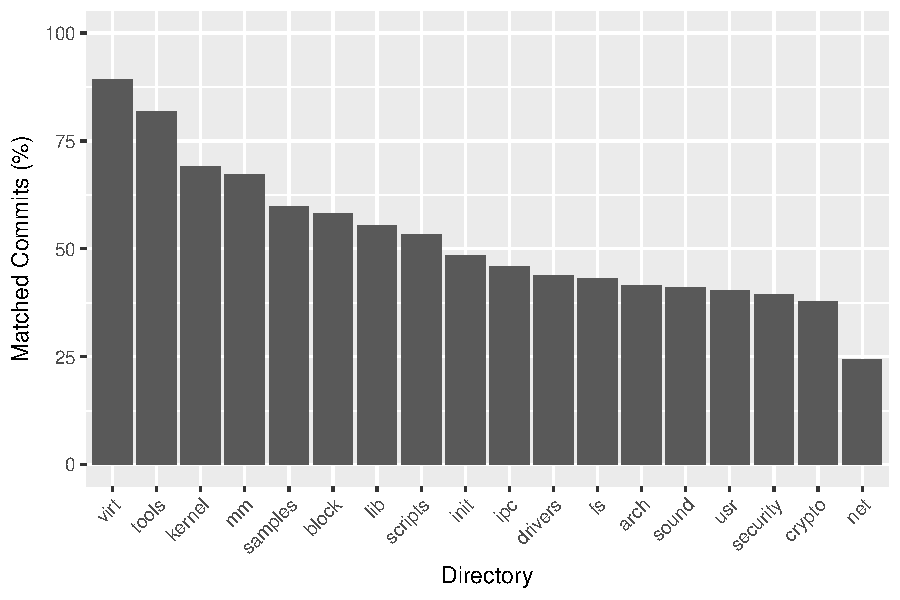
\includegraphics[scale=.6]{plots/matched_commits_dir}
  \caption{Percentage of matched commits in Linux subdirectories, from 2009 to the time of writing this paper.}
  \label{fig:matches_dir}
\end{figure}



%patch-based: \cite{msr13jojo,jiang14}
%actually, we're leveraging heuristic also mentioned by Jojo~\cite{jiang14} because nowadays it is standard practice <=> only from 2013 on? use only those in test

%\subsection{Formula for Historical Expertise}
%\label{sec:form-hist-expert}
%
%\begin{itemize}
%\item maybe, if too long to put in RQ2's approach
%\end{itemize}



\section{Case Study Results}
\label{sec:case-study-results}

This section discusses for each research question its motivation, specific approach and results.

\subsection*{RQ1. \rqone}
\label{sec:rq1.-how-does}

{\bf Motivation:} 

Open source software maintainers are responsible for the health of their subsystem. For example, each Linux kernel maintainer % ensures the healthy evolution of the Linux kernel
manages the changes proposed by developers to the subsystem they are responsible for, and shepherd those changes upstream towards the Git repository of Linus Torvalds (i.e., the official Linux kernel repository). Hence, their presence is vital to the kernel community.

Unfortunately, due to the unpredictable nature of life in general and open source software development in particular~\cite{Wu,Zhou}, maintainers, for various reasons, one day will be forced to give up their responsibilities. In most cases, this means that another developer will have to take over the responsibility of maintainer.

Hence, this research question aims to analyze how often maintainership changes in kernel development. Furthermore, we are interested in understanding how much of the code base of official releases is ``owned'' by the subsystem maintainers, i.e., was originally developed by a maintainer. Since ``git blame'' is a popular means for finding experts~\cite{Rahman-2011}, our results will help us understand to what extent such a measure is reliable to measure expertise.%  This allows to , as well as whether the workload of kernel developers also decreases over time \bram{if Zhou already found this, why are we doing it again? or is \texttt{legacy} measuring something else? if so, what is link with Zhou et al.'s work?}. \bram{did not get an answer about this, so removing it}% We investigate whether this decline in monthly workload and the decline in LOC footprint result in a loss of expertise.

{\bf Approach:}

To confirm the presence of changes in maintainership during the evolution of the Linux kernel, we analyzed the maintainers recorded in the \texttt{MAINTAINERS} file of releases \textit{v3.5} to \textit{v4.11} to identify how often maintainers (dis)appeared. % We compare the list of maintainers for each subsystem listed in the \texttt{MAINTAINERS} files contained in both releases of the linux kernel and count the number of subsystems where changes occured.
Furthermore, for each studied release, we measure and plot these maintainers' \texttt{legacy}, which corresponds to the number of surviving code lines of a maintainer, as given by ``git blame''. %understand the evolution of the LOC footprint of maintainer across time, we look at the "blame count" of each maintainer in each main linux release of the past 5 years. The blame count only contains the \textit{visible} lines of code associated with the maintainer in the files belonging to their subsystem.
We then validated the statistical significance of the change in \texttt{legacy} distribution between the first and last analyzed release using a Wilcoxon paired test. % between the \texttt{legacy} distribution of maintainers active in the studied period of .  
% list1=[across all maintainers of their \%lines owned in earliest release for given subsystem]
% list2=[same, in final release for which we have data for that person]
In case of a significant test result, we also provide the Cliff Delta effect size~\cite{Romano:2006}. An effect size smaller than 0.147 is deemed a ``negligible'' difference, smaller than 0.33 a ``small'' difference, smaller than 0.474 a ``medium'' difference and otherwise a ``large'' difference.


\begin{figure}[t]
  \centering
  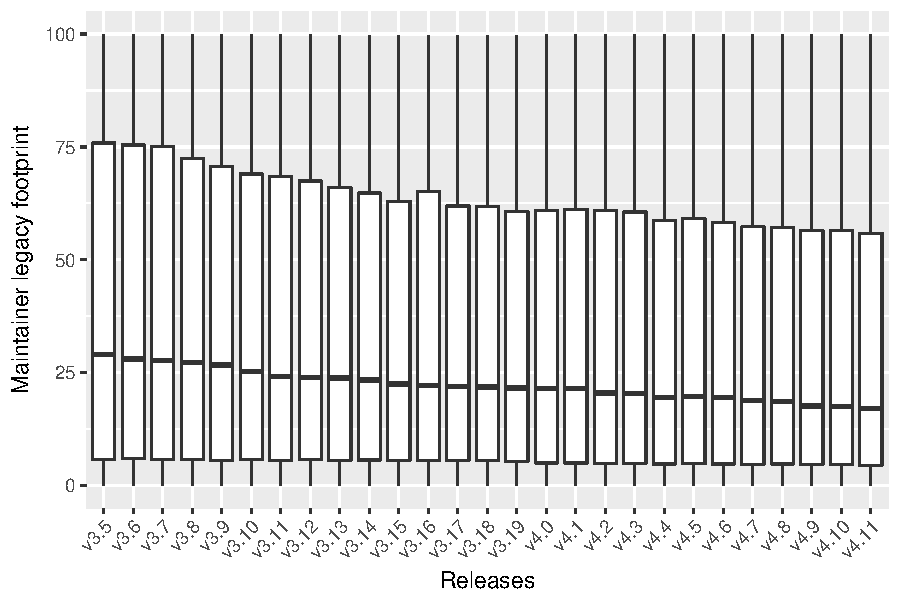
\includegraphics[scale=.6]{plots/RQ1_median_LOC}
  \caption{Median maintainer \texttt{legacy} across releases.}
  \label{fig:RQ1_temp}
\end{figure}

{\bf Results:}

\textbf{23\% of the studied subsystems saw changes in maintainership over the last 5 years.} Out of the 734 subsystems studied for RQ1, we counted 168 subsystems that experienced some sort of maintainership change. We counted 100 maintainer arrivals, 63 departures, and 88 replacements. These numbers confirm that maintainership change is common, even in mature open source systems like the Linux kernel. Furthermore, the median percentage of developers who are maintainers in the analyzed subsystems is 0.50\% (mean of 0.90\%), indicating that it is not straightforward to guess the next maintainer. These observations strengthen our case for more advanced expertise measures.

%\bram{do we have median plots now?}
\textbf{The median maintainer \texttt{legacy} significantly decreases over time.} \autoref{fig:RQ1_temp} shows the evolution of the median percentage of maintainer \texttt{legacy} across all subsystems in each studied release. The plot shows a clear, steady decrease of this measure across releases in terms of median and variance. We confirm the significance of this decrease with a Wilcoxon paired test ($\alpha=0.01$) between the first and last studied version, which yields a p-value of 2.2e-16.% We conclude that there is a significant decrease in LOC footprint during the observed period.


%\bram{no link at all with Zhou et al.'s work, it seems, as they? do we have better motivation? if not, leave out \autoref{fig:RQ1_temp}?}
Although the Cliff Delta value of 0.07 indicates only a negligible difference, this decreasing trend suggests that, if one limits the measure of expertise to the amount of surviving code originally authored by a maintainer, as was done by earlier work~\cite{Rahman-2011}, the expertise of maintainers globally seems to be decreasing over time. 

% \bram{no link at all with Zhou et al.'s work, it seems, as they? do we have better motivation? if not, leave out \autoref{fig:RQ1_temp}?}

%\bram{still don't understand the link with Zhou et al., so leaving it out} This finding mirrors those of Zhou et al.~\cite{Zhou-fse}, who have shown that the workload of Linux kernel maintainers over time is decreasing. This workload was defined by the number of files a maintainer is responsible for, the number of commits to those files authored by other authors, and the number of authors interacting with the maintainer. Not only is the total workload not evenly spread out across all maintainers, their monthly workload is decreasing as well.


%The     According to state of the art expretise metrics, this decline in LOC footprint should translate in a decline in expertise.
% \begin{itemize}
%   \item Number of subsystems experiencing maintainer changes over studied period: 168 / 734 = 22.8\%.
%   \item Wilcoxon text between first and last LOC footprint: paired: 2.2e-16 / without paired = TRUE : 0.02653
% \end{itemize}
%Wilcoxon test (paired!) between list1 and list2 => alpha value of 0.01
% scatterplot or hexbinplot plot(list1,list2) 

% \bram{I think we are also missing boxplots saying, for each release, the percentage of subsystem contributors that is maintainer; this is important to indicate how hard it is to find a maintainer, since a subsystem with only 2 contributors is super-simple to identify maintainers for} \alex{I just computed all the maintainer/developer ratios: median is 0.5 percent (in the 78 filtered subsystems), so the boxplot doesn't look very good.}\bram{is this median across all releases and subsystems?}

% I found the evolution of the median percentage of maintainers in their subsystem across all releases:  median of 0.5% is for all subsystems in the current release; mean is 0.9%

% release,percentage(%)
% 22,0.58170995671
% 21,0.534046345811
% 20,0.576080667824
% 19,0.583783049927
% 18,0.584750523467
% 17,0.597305919887
% 16,0.552486187845
% 15,0.574712643678
% 14,0.614125834666
% 13,0.6269377183
% 12,0.639506374632
% 11,0.646488699503
% 10,0.661158831115
% 9,0.694578429481
% 8,0.715749039693
% 7,0.739434694658
% 6,0.757586627448
% 5,0.784361975362
% 4,0.785857650146
% 3,0.82305920607
% 2,0.82372881356
% 1,0.85231394168


\subsection*{RQ2. \rqtwo}
\label{sec:rq2.-does-current}

{\bf Motivation:}

% important => currently state-of-the-art is based on code activity => evaluation shows it is far from perfect, so we check and see that priorities of people have changed

Prior work on expertise measures~\cite{Anvik-2006, Bhattacharya, McDonald, Minto-2007, mockus02} primarily are based on code activity, which can be defined in terms of \texttt{legacy} and \texttt{committed}% number of changes added to the source code (Commits)
. As motivated in \autoref{sec:expertise-formula}, we believe that these two metrics do not capture the full breadth of maintainer activities. Indeed, the results in RQ1 indicate that the \texttt{legacy} of long-standing maintainers crumbles over time. Unless one assumes that this reflects a real drop in expertise over time, the only explanation is that existing experts reorient their focus to other activities, such as code review and email communication. Hence, this research question evaluates whether considering such additional activities is able to improve the identification of experts.%Other facets of software development are not reflected by those metrics. Important development activities such as code reviews and upstream committing are not portayed by lines of code and commit authors.

{\bf Approach:}

% To validate this technique, we need a proven expertise indicator. This indicator would help us confirm wether or not an expertise measuring approach is accurate. In the case of the linux kernel, we believe maintainership is a good expertise indicator. Maintainers are responsible of the health and sustainability of their subsystem. Developers often reached this position by demonstrating a long record of involvement in subsystem discussion and contributions. In other terms, they are regarded as experts in their subsystems by the community. 

% With the assumption that maintainers are experts in their subsystems, we can validate the expertise measured by our different approaches by comparing maintainership and high expertise score. 

% The naive expertise calculation requires two different data points. On one hand, we extract a list of subsystems as well as their current maintainers and the list of files contained in the subsystem. On the other hand, we create a line of code count for each developer.

% Git blame makes it easy to count each developer's line of code count. We execute git blame on each files in the linux source code. For each of those files, we created a ranking of developers in terms of lines of code. With the acquired subsystem file tree, we are capable of aggregating the line of code developer ranking to the subsystem level. 

% Furthermore, we are able to apply the same technique to aggregate the other metrics to the subsystem level. 

To validate the ability of the measures in \autoref{tab:metlin} to explain expertise, we evaluate how well the $footprint_j(\mathbb{A})$ measure involving those measures is able to identify the maintainers of Linux kernel subsystems. Those maintainers are the experts listed in the \texttt{MAINTAINERS} file of a kernel release.

For a given release and subsystem, %different heuristics dicussed in section \ref{sec:contribution-footprint} in term of ability to detect experts, we look for the presence of maintainers and their position in their subsystem's different rankings. 
%We assume that maintainers have more experience in \textit{their} subsystem than other developers active in this subsystem. Therefore,
we should find the maintainers in the top positions when ranked based on footprint values. The combination of activity measures $\mathbb{A}$ that is able to systematically yield the correct maintainers across subsystems and releases could be assumed to be a better indication of expertise. 

In particular, we calculate two performance metrics:
\begin{description}
\item[$POS_N$] \underline{P}ercentage \underline{O}f \underline{S}ubsystems for which at least one maintainer was ranked in the top N recommended candidates
\item[$POM_N$] \underline{P}ercentage \underline{O}f \underline{M}aintainers in the {\em whole} project who were ranked in the top N recommended candidates for their subsystem
\end{description}

For these performance metrics, N is a threshold that can be varied. Our case study uses thresholds ranging from 1 to 5. It is important to note that, if the number of maintainers of a subsystem is larger than N, $POM_N$ could be penalized. To avoid this, we slightly changed the definition of $POM_N$ to be calculated only for the maintainers of all subsystems with at most N maintainers, instead of for all maintainers of the whole project. For example, $POM_1$ measures the percentage of top-recommended maintainers of subsystems with at most 1 maintainer.%having said that, how do we explain that for top-N it says out of all projects with at most N maintainers, what is percentage of them in top-N?

To structure our analysis, we analyzed the performance of maintainer recommender involving only one metric of \autoref{tab:metlin}, then analyzed models involving all combinations of \texttt{legacy} with one of the other 4 measures, and finally one model with all measures combined. 
% We focus explicitly on models involving \texttt{legacy} because it is a commonly used measure ~\cite{Rahman-2011}, and hence we use its performance as baseline. %We excluded the 20 other combinations because we aim to analyze the impact of the different activities combined with \texttt{legacy}. \bram{basically: we chose A and B, because we chose A ...}
% \bram{why?}\alex{Too complicated to compute for such marginal returns?} \bram{no, we wanted to study the impact of different groups of metrics, i.e., blame, then commit info, then review info}

Since, for a given release, there is one $POS_N$ value and one $POM_N$ value, we calculate these metrics for each release, then study their distribution across the analyzed releases using boxplots. % Second, we also measure for each subsystem whether the top N ranking finds at least one of the subsystem's maintainers (since finding one maintainer is enough for someone trying to ask a question).%We establish thresholds of a maximum ranking position to validate wether a metric or combination of metrics is a good expertise indicator. In other words
\autoref{fig:rq2_1} and \autoref{fig:rq2_3} show for each analyzed $\mathbb{A}$ % the performance of each studied metric and combination of metrics for
the distributions of $POS_N$ for N=1 and N=3, respectively, across the 22 studied Linux releases, while \autoref{fig:rq2_1_many} and \autoref{fig:rq2_3_many} the distributions of $POM_N$ for N=1 and N=3, respectively. % the proportion of \textit{subsystems} with at least one correctly identified within the top N footprint values of the subsystems, across the 22 studied Linux releases. 
We only show the plots for N=1 and N=3, as for higher values of N the plots remain more or less stable.
% TODO: stress other approaches used by other papers as baseline (legacy, committed)
% TODO: what is distribution of footprint values per subsystem? 1 clear winner?


% We track the following metrics:
% \begin{itemize}
% \item Number of LOC 
% \item Number of commits as author
% \item Number of commits as committer
% \item Number of review emails/reviewed patches
% \item Number of Commit message attributions
% \end{itemize}


 
%\begin{itemize}
%\item git blame
%\item currently most active developers: number of commits since last release (total since beginning not practical, since those people away) <=> not that easy to calculate yourself (until Jonathan Corbet releases his report) + only new contributions
%\end{itemize}



\begin{figure*}[t]
  \centering
  \begin{minipage}[b]{\columnwidth}
    \centering
    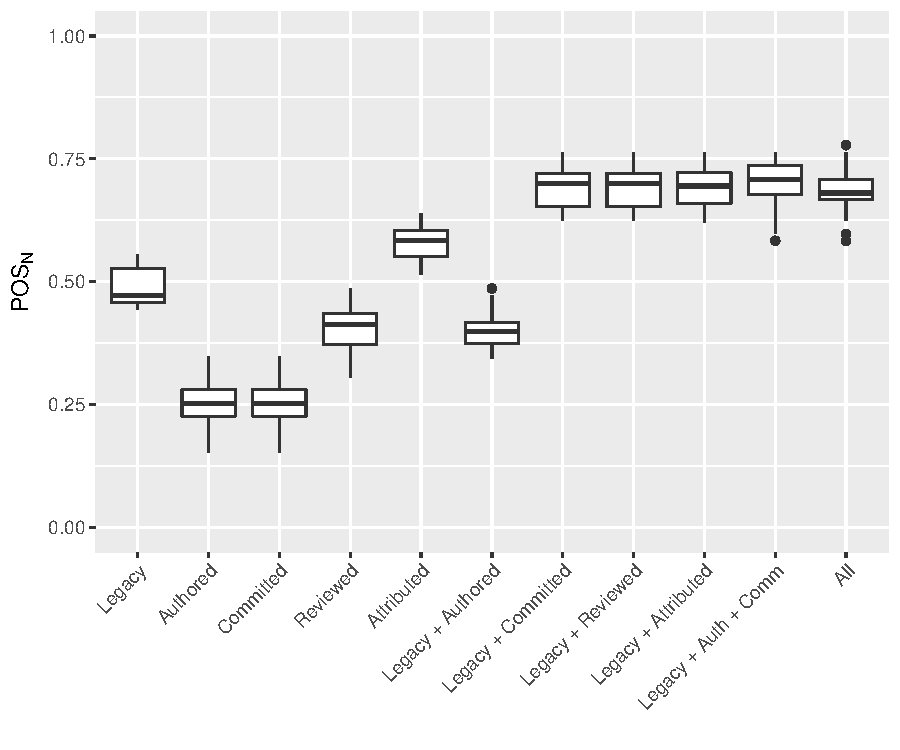
\includegraphics[scale=.5]{plots/RQ2_metrics_N1_one_maint}
    \caption{Distribution of $POS_N$ for each combination of activity measures, for ranking threshold N = 1. }
    \label{fig:rq2_1}
  \end{minipage}
  % \hfill
  \begin{minipage}[b]{\columnwidth}
    \centering
    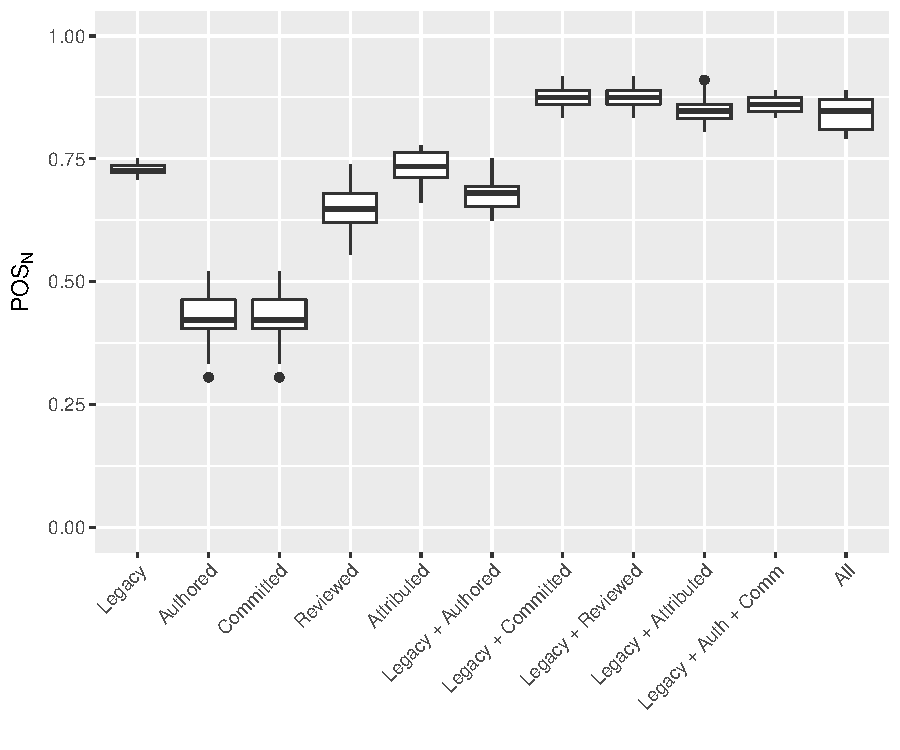
\includegraphics[scale=.5]{plots/RQ2_metrics_N3_one_maint}
    \caption{Distribution of $POS_N$ for each combination of activity measures, for ranking threshold N = 3. }
    \label{fig:rq2_3}
  \end{minipage}
\end{figure*}

\begin{figure*}[t]
  \centering
  \begin{minipage}[b]{\columnwidth}
    \centering
    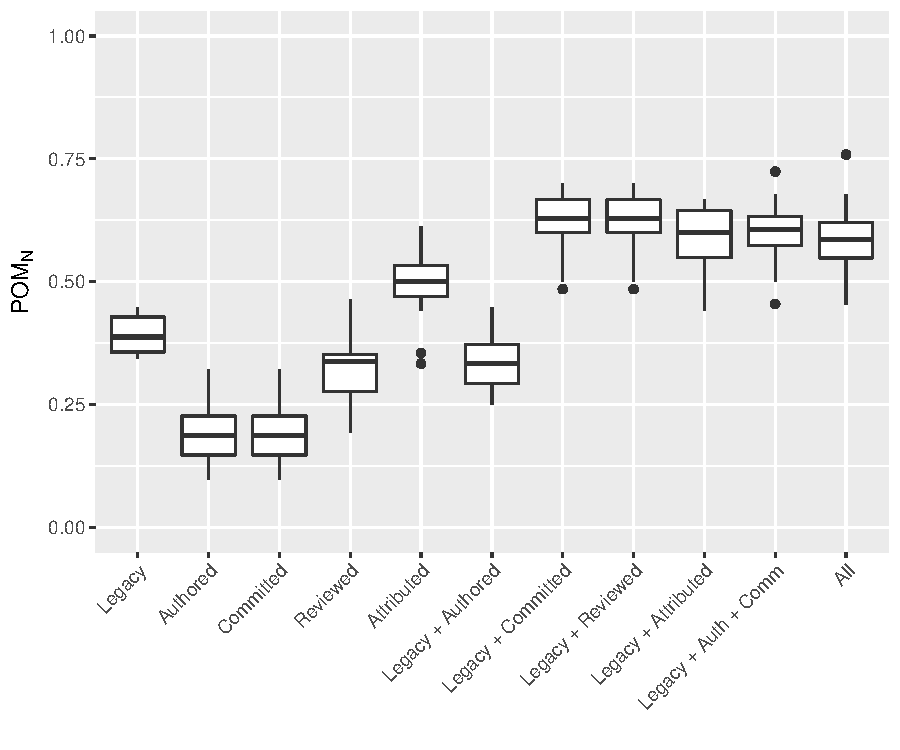
\includegraphics[scale=.5]{plots/RQ2_metrics_N1_many_maint}
    \caption{Distribution of $POM_N$ for each combination of activity measures, for ranking threshold N = 1. These boxplots only consider subsystems with at most 1 maintainer.}
    \label{fig:rq2_1_many}
  \end{minipage}
  % \hfill
  \begin{minipage}[b]{\columnwidth}
    \centering
    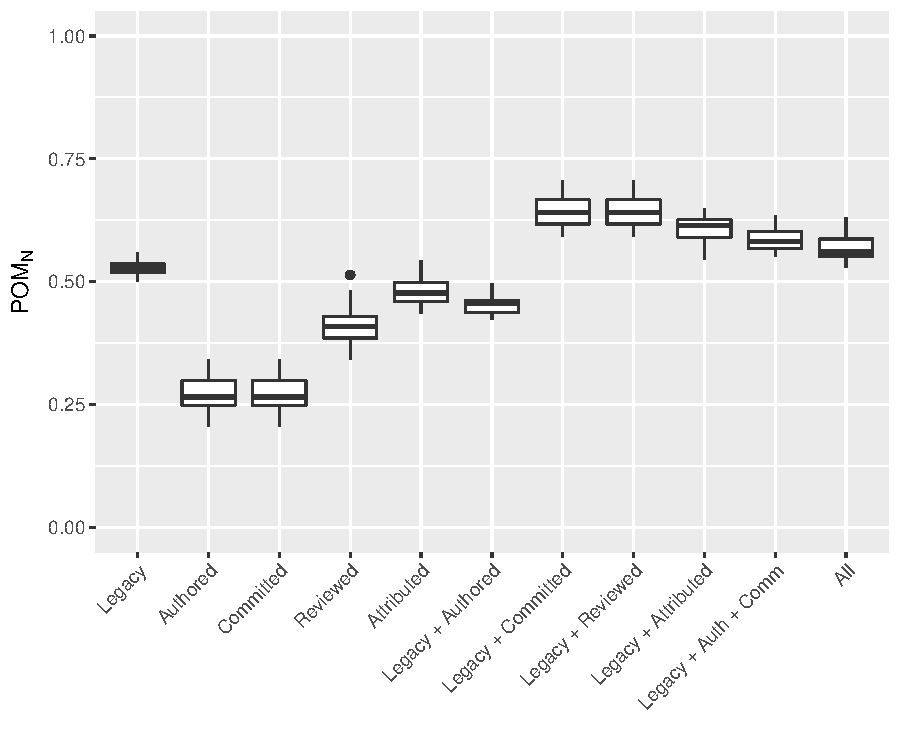
\includegraphics[scale=.5]{plots/RQ2_metrics_N3_many_maint}
    \caption{Distribution of $POM_N$ for each combination of activity measures, for ranking threshold N = 3. These boxplots only consider subsystems with at most 3 maintainers.}
    \label{fig:rq2_3_many}
  \end{minipage}
\end{figure*}



{\bf Results:}

\begin{table}[t]
\centering
 \begin{tabular}{c c c c c c c} 
 Type & Measure & N = 1 & N = 3 \\
 \hline
  $POS_N$ & P-value       & 4.27e-05 &  4.28e-05  \\
  $POS_N$ & Cliff's delta & 0.99    & 1.0     \\
  $POM_N$ & P-value       & 4.27e-05 & 4.77e-07  \\
  $POM_N$ & Cliff's delta & 0.84    & 1.0     \\
\end{tabular}
\caption{P-values and Cliff's delta values for the Wilcoxon paired tests ($\alpha=0.01$) between \texttt{attributed} and \texttt{legacy + committed} for ranking thresholds N=1 and N=3 and for $POS_N$ and $POM_N$.}
\label{table:rq2_wilc_att_loc_cc}
\end{table}

% After filtering out inactive and small subsystems, we are left with a subset of 78 subsystems. We ran the experiments with rankings thresholds from 1 to 5 on 22 different releases of the linux kernel (v3.8 to v4.11). 

\textbf{\texttt{attributed} is the only single-measure model able to keep up with the multi-measure models.} 

The results in \autoref{fig:rq2_1} and \autoref{fig:rq2_1_many} indicate that the first two individual measures, i.e., \texttt{legacy} and \texttt{authored}, are bad indicators of expertise compared to the other studied metrics. For example, in \autoref{fig:rq2_1}, \texttt{legacy} only reaches a median $POS_N$ value of 47.22\%, while \texttt{attributed} reaches a median $POS_N$ percentage of 58.4\%.

\textbf{The models combining \texttt{legacy} with \texttt{committed}, \texttt{attributed} and/or \texttt{reviewed} perform the best.} \autoref{fig:rq2_1} shows indeed how only these four models read median percentages of 69.9\%, while the other multi-measure models, especially the one involving only \texttt{legacy} and \texttt{authored}, are not able to outperform the best individual measure models. %The model becomes increasingly accurate when we build rankings based on a combination of metrics. These combinations allow for a wider representation of the different activities that make up linux kernel development.

These findings confirm the intuition that maintainers shifted focus from doing development (\texttt{authored}) themselves to mentoring others by controlling access to their subsystem's Git repository through committing and/or reviewing. As such, an expertise model only involving their own development (i.e., \texttt{legacy} and \texttt{authored}) is unable to explain the current kernel maintainers' expertise. In other words, modern expertise models should take into account the time spent reviewing code and pushing changes upstream.% should be accounted for in the implementation of an expertise measure.

% Combining different, unrelated metrics allows the model to compensate a decrease of one data point by an increase of another. For instance, a maintainer's decline in LOC footprint could be explained by an increase in code review, which would prevent the maintainer to contribute as much code as he used to. 

\textbf{$POS_N$ increases to a median of 87.5\% for larger N, with multi-measure models outperforming single-measure models by at least 17\%.} Comparing \autoref{fig:rq2_3} to \autoref{fig:rq2_1} shows how the top multi-measure models for N=1 are able to increase their distance compared to even the best single-measure models (\texttt{attributed}). This, compared with a change in best performing single-measure models, indicates that a larger diversity in activity measures enables better identification of the two additional candidate maintainers. Indeed, by considering top performing contributors across a wider range of activities, there is a larger chance at least one real maintainer is found. Although the percentages of \autoref{fig:rq2_1_many} and \autoref{fig:rq2_3_many} cannot be compared directly to each other (cf. modified definition of $POM_N$), \autoref{fig:rq2_3_many} (for $POM_N$) shows a similar ranking of models as \autoref{fig:rq2_1} (for $POS_N$), confirming the findings for $POS_N$.

\autoref{table:rq2_wilc_att_loc_cc} shows the p-value and effect size of the Wilcoxon test between \texttt{attributed} and \texttt{legacy + committed} for figures \ref{fig:rq2_1}, \ref{fig:rq2_3}, \ref{fig:rq2_1_many}, and \ref{fig:rq2_3_many}. Each effect size being close to 1, we notice a \textbf{large} performance increase between \texttt{attributed} and \texttt{legacy + committed}.

Interesting to note is that, across all analyzed releases, the boxplots show a remarkable small variance, especially for N=3. Although this is partially due to the fact that less than 25\% of the subsystems saw at least one maintainer change, it also indicates that our measures are stable across changes in the 5 activity measures used.%A metric combination that returns a higher than average accuracy is \textit{Lines of Code(LOC) + Commits Committer.} This proves that the decline in lines of code footprint does not indicate \textit{expertise erosion}, but rather, a shift in priorities between writting code and upstream committing??. 
% Maintainers are able to keep their level of expertise by staying involved 

%\begin{itemize}
%\item existing work looks at how much code still left in current version of code or how many commits done in latest release (cite papers): how does this expertise evolve across releases for each maintainer? => we will see drop
%\item why? they perform less commits, so their footprint on code is dropping + moving towards reviewing instead making commits themselves
%\item their code is eroding
%\end{itemize}



\subsection*{RQ3. \rqthree}
\label{sec:rq3.-does-historical}

{\bf Motivation:} 

% priorities seem to shift => add historical expertise + expertise in different activities (in particular code review, although there are other things we do not measure)
The metrics analyzed in RQ2 reveal that traditional expertise metrics
~\cite{McDonald,1572315,mockus02} based solely on a contributor's own development productivity are not well suited to identify maintainers. Expertise models exploiting only the information available for the release under study, are able to obtain median $POS_N$ performance of up to 75\% (N=1) and 90\% (N=3).%   first dimOther metrics, such as number of commits as a committer and number of commit message attributions are better indicators of maintainership. We believe this is due to a shift from development to reviewing activities. 

However, % the limitation of $footprint_j(\mathbb{A})$ is that it only accounts for the data found in the current release of the kernel. We
we believe that adding a historical dimension considering also the activity in the last R releases would assist the model in two ways. On the one hand, long standing kernel developers' contributions should carry more weight than newcomers' contributions. On the other hand, analyzing data on multiple releases would control for cases where contributors' productivity was lower due to a variety of reasons, such as illness, vacation or work on other projects.
%For these reasons, this research question evaluates the ability of the history-awaware $footprint_j^R(\mathbb{A})$ to explain expertise.
% The metrics used in RQ2 reveals a large difference between the existing measure of expertise and the official list of maintainers. We believe that this is due to the narrowness of the observed data points. As discovered in RQ1, maintainers have to focus their time on not only contributing to their subsystems, but also in reviewing the often large amount of patches being sent by other developers/contributors. We believe that this sort of activities should be accounted for in the implementation of an expertise measure. 





% looks at the number of code contributions for the latest observed Linux release (4.11). 

%previous RQ shows big gap between existing measures of expertise and official list of maintainers => reason: they ignore the erosion of expertise over time, where physical code presence slowly turns into more management-level activities => expertise does not vanish, just another form



{\bf Approach:}

%We tracked the different subsystems over a five year period. This allowed us to aggregate contributions, commits, and number of patches reviewed during the last 27 releases of the Linux kernel.
For each studied kernel release, we calculated $footprint_j^R(\mathbb{A})$ for R=4, since this covers a time span of 60 to 70 days. For example, when looking at experts in release \textit{v4.11}, we need to take into account data found for releases \textit{v4.7, v4.8, v4.9, v4.10, and v4.11}. We repeat such analysis for each of the 22 releases. In this paper, we use linearly decaying weights $W_i$ to combine the individual $footprint_j(\mathbb{A})$ values across the five considered releases, since this scheme is less extreme than the exponential and logarithmic ones.

Similar to RQ2, we then use the footprint values to create, for each subsystem and release, a ranking of all contributors active in the five considered releases% present in the last five release of the subsystem. We repeat this step for each studied subsystem and then for the last 22 releases
. We also use the same performance metrics as for RQ2, which allows us to compare the results of RQ3 to those of RQ2 to validate % .
% We can now apply the technique described in the approach of RQ2, and verify 
whether the historical dimension improves the model.

To save space, and since we found that, similar to RQ2, the combination of \texttt{legacy} and \texttt{committed} performs the best, we only show the results for this model (the rest of the data will be made available after the double-blind review). In particular, % maybe need exponentially decaying weights, where past counts, but newer stuff has higher weight
\autoref{fig:rq3_curr} and \autoref{fig:rq3_hist} show the $POS_N$ performance of the combined \texttt{legacy}+\texttt{committed} model without and with the history dimension, for ranking thresholds N ranging from 1 to 5. \autoref{fig:rq3_curr_many} and \autoref{fig:rq3_hist_many} show the corresponding $POM_N$ results.%\bram{also, did you double-check that this combined model is still the best one?} \alex{It is the best one, but it is already really good for the current percpective, so the performance increase is not as noticable when using historical. See table 3.} 

\autoref{table:rq3_wilc_loc_cc} contains the results of Wilcoxon paired tests between the $POS_N$ values without and with history, for each N, and (similarly) between the $POM_N$ values without and with history, for each N. For each test, we also provide the Cliff Delta effect size~\cite{Romano:2006}.% An effect size smaller than 0.147 is deemed ``negligible'', smaller than 0.33 ``small'', smaller than 0.474 ``medium'' and otherwise ``large''.

% To create rankings in a similar fashion as RQ2, we assign previous release data to linearly decaying weights. The data collected in \textit{v4.7} will carry less weight than the data found in \textit{v4.8}, as developers are less likely to lose experience acquired more recently \cite{Rigby}. 

% For each developer found in each tracked subsystem, we compute and weight the different metrics for the past 4 releases. For example: 

% \[
% \Big[M_{t-4}, M_{t-3}, M_{t-2}, M_{t-1}, M_{t} \Big]
% \]

% Where $M_t$ = the metrics collected for a developer in a given subsystem for release t. 

% \[
% W = \Big[0.2, 0.4, 0.6, 0.8, 1.0 \Big]
% \]

% \[
% Expertise Index = \sum_{t=1}^{5} M_{t} W_{t}
% \]

% ((( TODO: Cleanup equation)))


% need to filter data set based on number of maintainers, maybe their percentage of changed code/commits across time, ... => makes it more interesting for evaluation (harder to determine right answer)

% also need enough activity in subsystems that we study here, for example large enough percentage of releases in which they made at least one commit, or large enough average number of commits per release => maybe already do this at end of preliminary analysis?

\begin{figure*}[t]
  \centering
  \begin{minipage}[b]{\columnwidth}
    \centering
    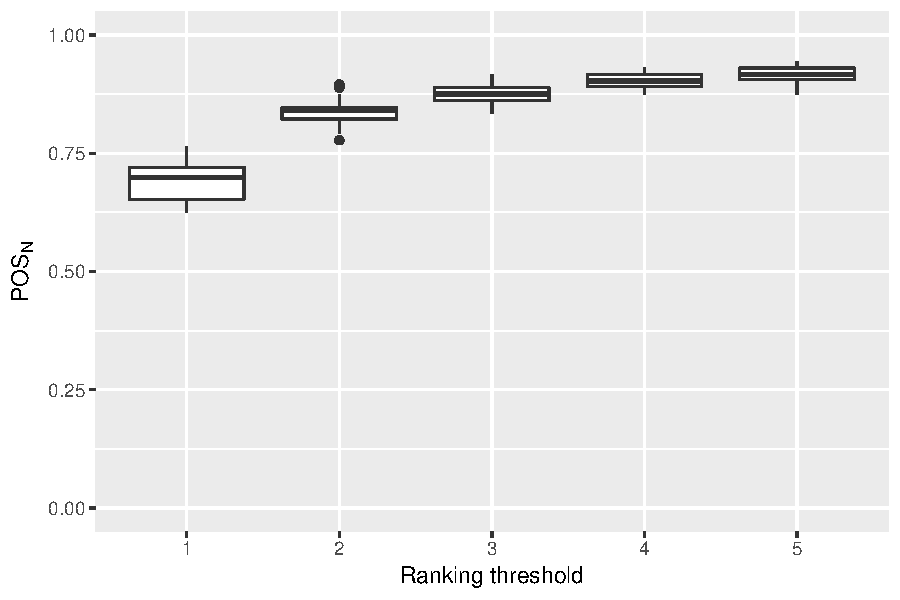
\includegraphics[scale=.5]{plots/RQ3_curr}
    \caption{Distribution of $POS_N$ for the combined \texttt{legacy}+\texttt{committed} model (\textbf{without} history dimension), for different N.}
    \label{fig:rq3_curr}
  \end{minipage}
  % \hfill
  \begin{minipage}[b]{\columnwidth}
    \centering
    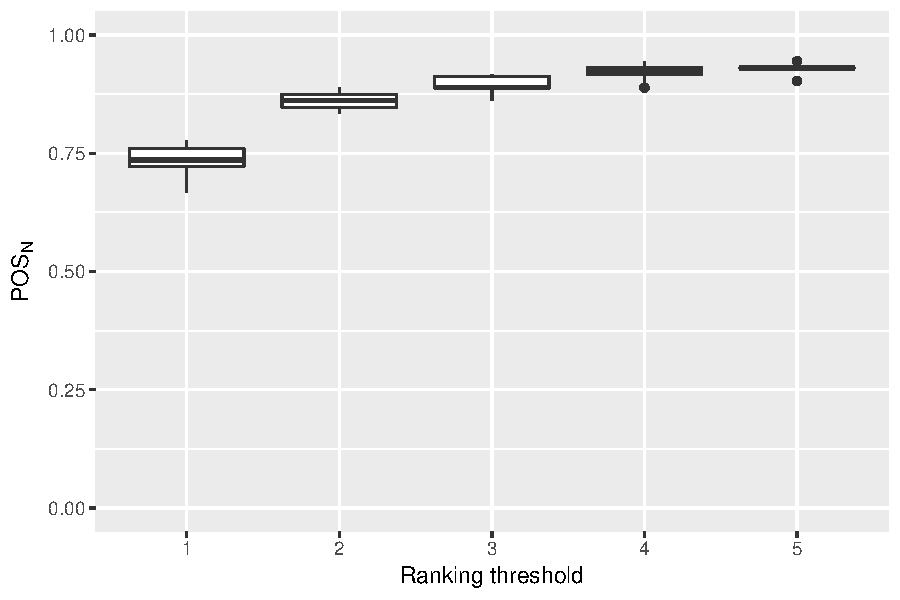
\includegraphics[scale=.5]{plots/RQ3_hist}
    \caption{Distribution of $POS_N$ for the combined \texttt{legacy}+\texttt{committed} model (\textbf{with} history dimension), for different N.}
    \label{fig:rq3_hist}
  \end{minipage}
\end{figure*}

\begin{figure*}[t]
  \centering
  \begin{minipage}[b]{\columnwidth}
    \centering
    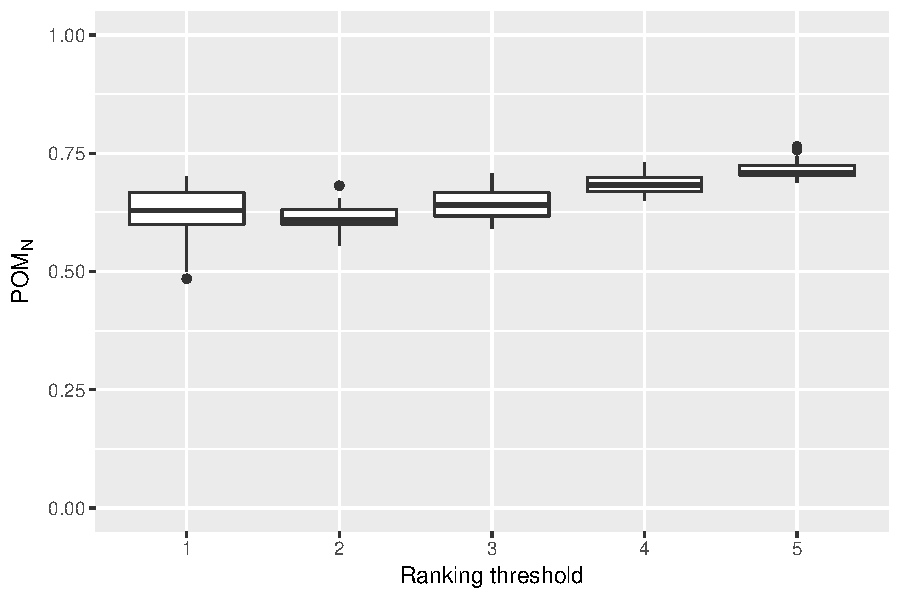
\includegraphics[scale=.5]{plots/RQ3_curr_many}
    \caption{Distribution of $POM_N$ for the combined \texttt{legacy}+\texttt{committed} model (\textbf{without} history dimension), for different N. For each N, the boxplot only considers subsystems with at most N maintainers.}
    \label{fig:rq3_curr_many}
  \end{minipage}
  % \hfill
  \begin{minipage}[b]{\columnwidth}
    \centering
    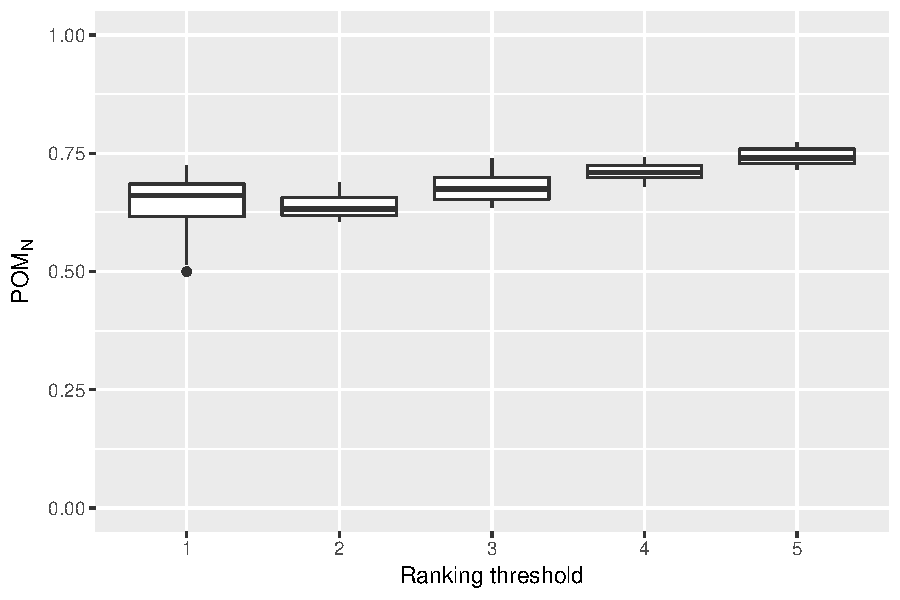
\includegraphics[scale=.5]{plots/RQ3_hist_many}
    \caption{Distribution of $POM_N$ for the combined \texttt{legacy}+\texttt{committed} model (\textbf{with} history dimension), for different N. For each N, the boxplot only considers subsystems with at most N maintainers.}
    \label{fig:rq3_hist_many}
  \end{minipage}
\end{figure*}



% \begin{table}[t]
%  \begin{tabular}{c c c c c c} 
%  Threshold N & 1 & 2 & 3 & 4 & 5 \\
%  \hline
%  P-value & 6.7e-05 & 5.7e-05 & 9.3e-05 & 2.1e-04 & 1.2e-04 \\
%  Cliff's delta & 0.6632 & 0.9442 & 0.7706 & 0.6384 & 0.6198
% \end{tabular}
% \caption{Cliff's delta and  p-values for the Wilcoxon paired tests between the performance results for the combined \texttt{legacy}/\texttt{authored}/\texttt{committed}, for ranking thresholds N=1 to N=5.}
% \label{table:rq3_wilc}
% \end{table}

\begin{table}[t]
 \begin{tabular}{c c c c c c c} 
Fig. & Measure & 1 & 2 & 3 & 4 & 5 \\
 \hline
\ref{fig:rq3_curr}/\ref{fig:rq3_hist} & P-value & 1.12e-4 & 8.76e-3 & 1.15e-2 & 1.57e-3 & 7.70e-4 \\
% \ref{fig:rq3_curr}/\ref{fig:rq3_hist}& Cliff's delta & 0.62 & 0.50 & 0.43 & 0.55 & 0.51 \\
      \ref{fig:rq3_curr}/\ref{fig:rq3_hist}& Cliff's delta & 0.62 & 0.50 & - & 0.55 & 0.51 \\
\ref{fig:rq3_curr_many}/\ref{fig:rq3_hist_many} &  P-value & 1.27e-2 & 4.63e-3 & 5.13e-4 & 1.57e-5 & 1.88e-4 \\
% \ref{fig:rq3_curr_many}/\ref{fig:rq3_hist_many}& Cliff's delta & 0.25 & 0.46 & 0.56 & 0.66 & 0.69 \\
   \ref{fig:rq3_curr_many}/\ref{fig:rq3_hist_many}& Cliff's delta & - & 0.46 & 0.56 & 0.66 & 0.69 \\
\end{tabular}
\caption{P-values and Cliff's delta values for the Wilcoxon paired tests ($\alpha=0.01$) between the $POS_N$ results of \autoref{fig:rq3_curr} and \autoref{fig:rq3_hist}, and of \autoref{fig:rq3_curr_many} and \autoref{fig:rq3_hist_many}, for ranking thresholds N=1 to N=5. A Cliff delta ``-'' indicates a non-significant test result, with p-value$>\alpha$}
\label{table:rq3_wilc_loc_cc}
\end{table}


% \begin{table}[t]
%  \begin{tabular}{c c c c c c} 
%  Threshold N & 1 & 2 & 3 & 4 & 5 \\
%  \hline
%  P-value & 0.01267 & 0.004634 & 0.0005127 & 1.574e-05 & 0.0001884 \\
%  Cliff's delta & 0.2479339 & 0.4607438 & 0.5640496 & 0.6590909 & 0.6942149
% \end{tabular}
% \caption{Cliff's delta and  p-values for the Wilcoxon paired tests between the performance results for $POM_N$ for the combined \texttt{legacy}/\texttt{committed}, for ranking thresholds N=1 to N=5.}
% \label{table:rq3_wilc_plot9_10}
% \end{table}



{\bf Results:}

\textbf{The history-aware \texttt{legacy}+\texttt{committed} footprint models perform significantly better than the history-unaware models.} \autoref{fig:rq3_curr} and \autoref{fig:rq3_hist} show how, except for N=3, the median performance of the history-aware expertise measure improves upon the history-unaware measure. If one considers only the first recommendation of the measure, there is a median 73.6\% chance that at least one maintainer is identified for a history-aware expertise model compared to 69.9\% with the single-release model. This difference progressively decreases for higher N, which means that, for higher N, an expertise model considering \texttt{legacy}+\texttt{committed} on one release only is robust enough to assess expertise.

We find similar improvements for \autoref{fig:rq3_curr_many} and \autoref{fig:rq3_hist_many}, except that the improvements due to history increase for larger N (and for N=1 there is no significant improvement). This is clearly shown % The differences in performance between the models without and with history are significant, as is shown 
by the p-values and effect sizes of the Wilcoxon paired tests in \autoref{table:rq3_wilc_loc_cc} ($alpha=0.01$). As an effect size greater than 0.474 indicates a \textbf{large} increase in performance, we notice that 7 of the 8 significant differences have an effect size of at least 0.50. %Since all the resulting p-values are under 0.01, we safely reject $H_0$ and accept $H_1$. (((Revisit)))
%\bram{can we add more discussion here and in RQ2 about the subsystems for which performance was better/worse than other subsystems?}


\section{Discussion}
\label{sec:discussion}

\textbf{Threats to validity:}

Threats to external validity prevent generalization of empirical results to other contexts. In particular, due to the abundant volume of data and presence of an oracle for expertise, our empirical evaluation only focused on 22 releases, or five years of the Linux kernel project. Hence, the study should be expanded to cover not only more kernel releases, but also other open (and closed) source projects. Furthermore, we considered only 5 expertise measures for our footprint models. Other measures, such as those mentioned in \autoref{tab:met}, should be studied to understand their impact on expertise.
% \begin{itemize}
% \item only Linux kernel
% \item only 22 releases
% \item only 5 measures
% \end{itemize}

Threats to construct validity involve risks regarding the measures used in the empirical study. Of the five considered expertise measures, \texttt{reviewed} was the only one requiring noisy approximations. Except for cases where the email patch subject was identical to the Git commit message summary, there is a definite risk of false positive and false negative matches, as identified earlier by Jiang et al.~\cite{msr13jojo,jiang14}. This might explain the relatively weak performance of expertise models involving \texttt{reviewed}. However, no better alternatives exist for projects that use mailing lists for code review. Projects using web-based review environments like Gerrit do not have this issue, and will have perfect matching between commits and their reviews.
% construct:
% \begin{itemize}
% \item matching not perfect => sub-par performance of review-related metrics could be explained by this
% \end{itemize}

Finally, regarding threats to internal validity (i.e., confounding factors potentially explaining our findings), we mention the limited number of subsystems considered for RQ2 and RQ3. This number was the result of the data filtering in \autoref{sec:data-filtering} used to eliminate temporarily inactive subsystems. Furthermore, we used the \texttt{MAINTAINERS} file as oracle for expertise. Although this is the known reference in the Linux kernel community for finding the right maintainer to contact, this is a manually maintained text file that hence could contain inconsistencies (even though changes to it are peer-reviewed).

Finally, although maintainership is a form of expertise, there are other forms of expertise that our footprint models be indicators of that were not considered in our empirical study. As such, some of the false positive recommendations of our footprint rankings might actually be correct suggestions based on a different interpretation of expert, in which case our $POS_N$ and $POM_N$ results are lower bounds for the actual performance.
% internal:
% \begin{itemize}
% \item limited number of subsystems for RQ2 and RQ3 due to filtering
% \item using kernel maintainers as experts
% \end{itemize}


\textbf{Future work:}

Apart from addressing the threats to validity, other future work should consider different weights $w_i$ and $W_i$. The former weights consider different activities to be more relevant than others, while the latter weights would give more or less weights to older vs. newer releases. For example, comparison of exponential and logarithmic decaying weights to the linear decay used in our study could be interesting. Similarly, different values of $R$ for $footprint_j^R(\mathbb{A})$ should be evaluated.

%Deeper analysis of email reviews

%Additional activity measures, such as churn, regular email activity, etc.

%Manually identify experts who are not necessarily maintainers, and use them to further validate model

%future work: alternative approach would be to look at characteristics of experts and those becoming new maintainer, then explanatory model to find major characteristics (we instead did a constructionist approach)
Finally, whereas we used a top-down approach from expertise model to evaluation on an actual open source project, a bottom-up approach starting from the analysis of a project's or subsystem's maintainers before formulating expertise measures and models could provide complementary insights into different kinds expertise.

%other systems than Linux

%look at distribution of each measure, then transform in specific way in order to best separate values (e.g., also filtering too low values, ...)


\section{Conclusion}

This paper argued about the need for expertise models considering a wide range of developer and other activities, and doing so across different snapshots of a project instead of just for one snapshot. Through an empirical study on 22 releases of the Linux kernel, we empirically showed how measures about a maintainer's own coding footprint (\texttt{legacy}) and her involvement in coordinating other project members (e.g., committing their commits and/or reviewing their code changes) significantly improves on coding-only expertise models for the sake of maintianer recommendation. Furthermore, considering those measures across different releases significantly improved performance, with large effect size.

The simplest incarnation of our maintainer recommender that software organizations should consider adopting involves (1) a developer's code \texttt{legacy} and number of changes \texttt{committed}, which are both readily obtainable from a Git log, calculated across (2) the last 5 releases. In future work, we will consider additional activity measures and empirically analyze other open source projects.




             % Troisième thème (Doctorat) ou effacez ce fichier si vous êtes à la Maîtrise.
\Chapter{CONCLUSION}
\label{sec:Conclusion}


The research project described in this thesis establishes a history-aware model capable of predicting experts in a large software project. We describe the different metrics acquired for the creation of the model as well as the techniques used to mine the necessary data. We were able to make some of the data available to the Linux community through two open source tool available online. We describe the different steps undertaken during the deployment of those tools. We also provide an evaluation of our expertise model.


\section{Advancement of Knowledge}


In addition to communicating our findings regarding expertise models in a submitted scholarly article, we were able to build two interfaces to further share our data with the rest of the Linux community. The main advancement of knowledge carried by our research project is the new dimentions used in our expertise model. State of the art techniques fail to include other aspects of software engineering, like code reviews and upstream committing. Our model is more appropriate to large organization where mainainers or managers are usually too busy to continue contributing code to the project. 

\section{Limits, Constraints, and Recommendations}
\label{sec:Limits and constraints}



\subsection{Srcmap}

Srcmap, our visualization of the kernel and its authors, has a few constrains and a lot of possible future work. The main constrain is the lack of a fluid user experience. The amount of data to process in the browser is too high to allow smooth browsing of the main tree. A way to address this issue would be to configure the interface to only download the required data as users browse the visualization. This way, the internet browser uses to display the tool would not have to save the entire dataset in memory and would only process the desired area. 



\subsection{Email2git}

Email2git, our code reivew tracking system, has a few important limitations. The first limitation to consider is the missing mailing list. Although our patch data source, patchwork.kernel.org, already track many mailing lists, some major mailings list like \texttt{net-dev} are not tracked. This is reflected in the low number of commit matched in the \texttt{net} subdirectory. 

We recieved a lot of valuable feedback from linux developers after our refereed talk the Open Source Summit North America. A developer mentioned the absence of the \textit{Patch 0} from our current implementation of Email2git. The Patch 0 is a summary of the changes submitted, often in multi-patch submissions. Another suggestion was to track \textit{linux-next}. This would allow developers to access discussion behind commits that have not been integrated in the main tree. 

For the future of this project, we recommend running our own instance of Patchwork 2.0, which automatically track the Patch 0 of each patch. In addition to ansering the lack of Patch 0, it would allow to have control on the tracked mailing lists. If we have access to old archives of the desired mailing lists, we could be able to create matching data dating to before 2009. We also recommend tracking the linux-next tree, as Email2git could ease the integration debugging process. 


\subsection{Paper}

There are two main limitation to the model proposed in our submitted paper. The first limitation is a direct concequence of Email2git's limitation. The missing mailing lists cause an uneven distribution of the matched commits accross the different subdirectories of the kernel. To address this limitation, we only studied subsystems with a certain percentage of matched commits. This ensured homogeneity of the data among the different subsystems. 

The other limitation is the validation technique we implement to assess the performance of our model. We use the maintainers currently active in the subsystem for the studied release. The issue with the technique is that since our model is partially based on activities usually related to maintainership, such as code reviews and upstream committing. To evaluate our model as \textbf{maintainer recommender} instead of an \textbf{expert recommender}, we would have to look at the developers that were selected as a replacement for a departing maintainer. A strong model would be capable of detecting the chosen developer for the release before the maintainer change.

At last, we cite the existing link between code stability and knowldge of that code area. Since our model offers a customaizable historical weight function, we could choose this weight function according to the stability of the code. For example, we could implement an exponential weight function to a very stable code base, as older contributions should account for more of the expertise measure. Furthermore, a code base undergoing large amounts of changes could require a logarithmic weight function, as older contributions should not affect current expertise as much as recent contributions. 



         % Conclusion.
%\backmatter
\renewcommand\bibname{REFERENCES}
\bibliography{Document}
%\bibliographystyle{polymtl}  % Format de la bibliographie.
\bibliographystyle{IEEEtranSN-francais}  % Format de la bibliographie.
%
\ifthenelse{\equal{\AnnexesPresentes}{O}}{
\appendix%
\newcommand{\Annexe}[1]{\annexe{#1}\setcounter{figure}{0}\setcounter{table}{0}\setcounter{footnote}{0}}%
%%
%%  Annexes.
%%
%%  Note: Ne pas modifier la ligne ci-dessous.
\addcontentsline{toc}{compteur}{APPENDICES}
%%
%%
%%  Toutes les annexes doivent être inclues dans ce document
%%  les unes à la suite des autres.
\Annexe{DEMO}
Texte de l'annexe A\@. Remarquez que la phrase précédente se termine
par une lettre majuscule suivie d'un point. On indique explicitement
cette situation à \LaTeX{} afin que ce dernier ajuste correctement
l'espacement entre le point final de la phrase et le début de la
phrase suivante.


\begin{landscape}
\Annexe{ANOTHER APPENDIX}
Text in «landscape» mode. 
\end{landscape}

\Annexe{ONE MORE APPENDIX}
Text.
}{}
\end{document}
